%\documentclass[12pt]{article}
\documentclass[12pt,preprintnumbers,nofootinbib]{revtex4}
%\documentclass[draft,12pt]{article}
\usepackage{amsmath}
\usepackage{amsfonts}
\usepackage{amsbsy}
\usepackage{lscape} 
\usepackage{color}
\usepackage{graphicx,epsfig}
\usepackage[english]{babel}
\usepackage{latexsym}
\usepackage{amssymb}
%\usepackage{palatino}
%\usepackage{chancery}
%\usepackage{newcent}
%\usepackage{charter}
%\usepackage{zapfchan}
%\usepackage{bookman}
%\usepackage{sparticles} 	%Package for displaying sparticle names. 
%\usepackage{feynmf}		%Package for feynman diagrams. 

%% slashed symbols
%\newcommand{\slashed}[1]{\hbox{{$#1$}\llap{$/$}}}
%\newcommand{\sslashed}[1]{\hbox{{$#1$}\llap{$/\,$}}}

\newcommand{\beq}{\begin{equation}}
\newcommand{\eeq}{\end{equation}}

\newcommand{\p}{\partial}
\newcommand{\wt}{\widetilde}
\newcommand{\ov}{\overline}
\newcommand{\md}{\mathcal{D}}

\newcommand{\suc}{{{\rm SU}_{\rm C}(3)}}
\newcommand{\sul}{{{\rm SU}_{\rm L}(2)}}
\newcommand{\ue}{{{\rm U}(1)}}
\newcommand{\el}{{\rm EM}}
\newcommand{\GeV}{{\rm GeV}}
\newcommand{\uflavor}{\mathbf{1}_{\rm flavor}}
%\newcommand{\su3}{{\rm SU}_{\rm C}(3)}
\newcommand{\lgr}{\left\lgroup}
\newcommand{\rgr}{\right\rgroup}

%\newcounter{dim5}
%\setcounter{dim5}{5}


\begin{document}


%%
%% The title page
%% 
%\begin{titlepage}
\renewcommand{\thefootnote}{\fnsymbol{footnote}}

%\hspace{-4cm}
%\begin{center}
%{\Large
%  \textbf{
%  \textsc{Classification of Dimension 5 Lorentz Violating Interactions 
%		in the Standard Model}
%         }
%      }

\title{Classification of Dimension 5 Lorentz Violating Interactions 
		in the Standard Model}
%\title{$\;\;\;\;\;\;\;\;\;\;\;\;\;$
%Electric Dipole Moments as Probes of $CPT$ Invariance $\;\;\;\;\;\;\;\;\;\;\;\;\;$}


\author{Pavel A. Bolokhov$^{\,(a,b)}$ and Maxim Pospelov$^{\,(a,c)}$}


\affiliation{$^{\,(a)}${\it Department of Physics and Astronomy, University of Victoria, 
     Victoria, BC, V8P 1A1 Canada}\\
$^{\,(b)}${\it Theoretical Physics Department, St.Petersburg State University, Ulyanovskaya 1,
        Peterhof, St.Petersburg, 198504, Russia}\\
$^{\,(c)}${\it Perimeter Institute for Theoretical Physics, Waterloo,
Ontario N2J 2W9, Canada}
}


%\vspace*{3.0cm}
%\begin{center}
%{\Large
%  \textbf{
%  \textsc{Classification of Dimension 5 Lorentz Violating Interactions 
%		in the Standard Model}
%         }
%      }
%
%\vspace*{1.0cm}
%  {\large \fontfamily{ppl}\selectfont Pavel A. Bolokhov~ 
%	{\normalsize\bf \textsc{and}} ~Maxim Pospelov}
%
%\vspace*{1.5cm}
%{\large\bf Abstract}
%%	We introduce Lorentz violating interactions at dimension five level into
%%	the Standard Model.
%\end{center}

\begin{abstract}
	We give a complete classification of mass dimension five Lorentz-noninvariant interactions
    composed from the Standard Model fields, using the effective field theory approach. 
    We identify different classes of Lorentz violating operators, 
    some of which are protected against transmutation 
    to lower dimensions due to the quantum loop effects. Within each class of operators we determine  
    a typical experimental sensitivity to the size of Lorentz violation. 
\end{abstract}
	
	

%	We demonstrate a method how to systematically extend a theory with
%	Lorentz violating interactions on the example of the Standard Model.
%	Starting with QED we build the Lagrangian which exhibits the basic
%	features of a LV theory, and derive the RG flow equations for its
%	parameters.
%	In a similar fashion we proceed with the Standard Model and provide
%	a full list of LV interactions. 
%	We discuss typical experimental constraints applicable to the parameters
%	of such a theory.

\maketitle

%\end{titlepage}

%\newpage
%
%\tableofcontents

\newpage


%	The idea of possible inexactness of the Lorentz symmetry has
%	been proposed long ago [{\it a ref here}].
%	Justifications of why it might be so originate from such 
%	popular directions as loop gravity theory, string theory and 
%	lattice models.
%	The quest for {\it violation} of the Lorentz symmetry one
%	may treat in two ways. 
%	First, this is a fair test of a fundamental symmetry of the
%	nature which lies at the origins of the field theory.
%	On the other hand, should a deviation be found, it would be a 
%	direct sign of new physics, such as any of the models mentioned 
%	above or other models suggesting Lorentz violation (LV).
%
%	So far, Lorentz invariance has passed the test. 
%
%	To describe a Lorentz-violating theory we use the Effective
%	Field Theory framework.
%	In this framework, having a UV theory, one can integrate 
%	the high-energy degrees of freedom arriving to a low-energy
%	{\it effective} field theory. 
%	The low energy theory can be identified {\it e.g.}
%	as the Standard Model.
%	However, besides usual gauge and Yukawa couplings, the 
%	effective theory will contain higher dimensional interactions	
%	--- the remnants of the UV theory.
%	Were we to know the physics of the UV theory, we would have
%	been able to predict the higher dimensional (irrelevant) 
%	corrections.
%	But the problem at hand can be speculatively formulated inversely: 
%	given the set of the irrelevant operators --- what physics
%	would they correspond to?
%	Or, speaking more strictly, given the constraints on the
%	irrelevant operators, can we infer any constraints on some of the
%	models of UV physics?
%	This is what the EFT gives the answer for.
%
%	Indeed, the Lorentz symmetry, should it be inexact, cannot
%	be violated strongly.
%	Therefore, it is fair to consider an LV model to be an exact
%	Lorentz invariant theory, which has been modified by tiny
%	LV corrections.
%	These corrections are the signature of the new physics governing
%	at the UV scale, and in the framework of the EFT, 
%	should be considered as the irrelevant operators.
%	In order to contain an amount of Lorentz violation, these operators
%	must be coupled to a constant vector (or tensor) background.
%	The mass dimension of these interactions then provides a natural
%	scale of magnitude (or importance) for them, 
%	since in the EFT an operator of a mass dimension $ d $ must be 
%	suppresed by a factor of $ \Lambda_{\rm UV}^{d-4} $.
%	
%	It is then instructive to consider a general field theory lagrangian
%	with arbitrary interactions coupled to arbitrary constant tensors,
%	added order by order with respect to their mass dimension.
%	If present, the highest importance will be brought by the 
%	{\it relevant} operators --- those of mass dimension three or
%	less if any. 
%	They would be enhanced by $ \Lambda_{\rm UV}^{4-d} $.
%	Then come the marginal operators, of the dimension four.
%	After them come the operators of mass dimension five, six, etc.
%	{\bf some examples here are desired.}
%	
%	Considering such corrections provides a smooth transition
%	between a theory with a hard broken Lorentz symmetry and a theory 
%	where the Lorentz invariance is softly broken --- {\it i.e.}
%	such theories are examples of the most general violation of Lorentz
%	symmetry.
%	Indeed, a theory with a hardly broken Lorentz symmetry is a
%	theory where the Lorentz symmetry is not present at all. 
%	In other words, if there are vector or tensor fields in the theory,
%	they totally do not care that the lagrangian should be a scalar 
%	--- this is just a theory where there is no restriction that
%	the Lorentz indices be contracted in the lagrangian.
%	The lagrangian is then just a sum of a number of terms where
%	the Lorentz index is being treated a just a mere ``index'' of a field:
%\begin{equation*}
%   {\bf an example here.}
%\end{equation*}
%	But what if we perform a Lorentz boost? 
%	The terms will rotate
%	and change their appearance and so will the lagrangian. 
%	That means that besides writing down the lagrangian one should
%	also specify which {\it frame} it is being defined in ---
%	the theory is only valid in a specific frame.
%	But that is fair since we do not have the symmetry which connects
%	all the inertial frames any longer.
%	If one wants to define an equivalent theory in a different frame,
%	he or she will have to write a different lagrangian.
%	But the rules of a transition from one frame to another are exactly
%	the same as if our interactions were contracted with constant
%	tensors, which also transform as we pass from frame to frame.
%	That means that a {\it generic} Lorentz non-invariant theory
%	can be described by a still Lorentz-invariant lagrangian which 
%	is made up of various interactions coupled to arbitrary
%	tensor backgrounds.
%
%	In a theory where the Lorentz invariance is broken spontaneously,
%	one or more vector (or tensor) fields acquire vacuum expectation
%	values, and become the background tensors coupled to, generically,
%	operators of various dimensions. 
%	Since the Lorentz symmetry violation is widely shown to be
%	less than miniscule and therefore can be treated as a perturbation, 
%	if it still exists it is more probable to be
%	violated spontaneously rather than totally absent in the UV theory.
%	The difference between a ``perturbed'' theory and a theory
%	with hardly broken Lorentz symmetry is that in the former one the
%	background tensors are appreciably small in magnitude, 
%	whereas in the latter case they can be of the order one ({\it i.e.}
%	comparable with the kinetic term) or even unlimited.
%
\section{Introduction}

%	Violation of Lorentz invariance has more often become one of the
%	ingredients or properties of low energy effective models.
	
	Lorentz symmetry is one of the most important ingredients of the 
	Standard Model (SM) of particles and fields, as well as its extensions at the 
electroweak scale. Even though there is a robust evidence that Lorentz symmetry is maintained to a 
high degree of accuracy, the searches of the so-called "Lorentz Violation" (LV) 
are still well-motivated. The reason is that an a priori unknown physics at high 
energy scales could lead to a spontaneous breaking of Lorentz invariance by 
giving an expectation value to certain non-SM fields 
that carry Lorentz indices, such as vectors, 
tensors, and gradients of scalar fields. The interaction of these fields with  operators composed 
from the SM fields, fully Lorentz-symmetric before the spontaneous breaking, below the 
scale of the condesation will manifest itself as effective LV terms. Schematically, one 
has 
\begin{equation}
O^{\rm SM}_{\mu\nu...} C^{\mu\nu...} \to O^{\rm SM}_{\mu\nu...} \langle C^{\mu\nu...} \rangle,
\label{start}
\end{equation}
where $C^{\mu\nu...}$ is an external field that undergoes condensation, and 
$O^{\rm SM}_{\mu\nu...} $ is the SM operator that transforms under 
the Lorentz group. It would be fair to say that the dynamical breaking of Lorentz 
invariance is difficult to achieve in a consistent UV-complete theory, and most of the 
papers studying LV shy away from this issue. 
 Nevertheless, the spurion or the effective field theory approach has been instrumental in 
comparing the sensitivty of various LV tests. 
	
If the generation of interaction \eqref{start} is a true UV phenomenon, it proves extremely useful 
to classify all operators of lowest dimensions coupled to a given spurion field $	C^{\mu\nu...}$.
At dimension three and four levels, this was done nearly a decade ago by Kostelecky and co-workers. 
Dimension three Lorentz violating interactions, {\em e.g.} $b^\mu \psi i\gamma_\mu\gamma_5\psi$ and 
 $a^\mu \psi i\gamma_\mu\psi$, must defy the naive dimensional counting, according to which $
 a^\mu$ and $b^\mu$ scale linearly with the UV energy scale responsible for LV, 
$a^\mu,b^\mu \sim \Lambda_{UV}$. This is, of course, in a stark contradiction with reality, 
where typical values for {\em e.g.} $b_\mu$ of light quarks are known to be smaller than 
$10^{-31}$ GeV. It can be hypothesized that spurions at dimension three and four levels are in fact 
not fundamental, but indeed effective, implying a different type of scaling, {\em e.g.} 
$a^\mu,b^\mu \sim \Lambda_{\rm IR}^2/\Lambda_{\rm UV}$, where $\Lambda_{IR}$ is the energy scale 
associated with the SM. The appearence of $\Lambda_{UV}$ in the denominator implies that above the 
scale $\Lambda_{\rm IR}$ one should be able to formulate all LV interactions in terms of the  
{\em higher-dimensional} LV operators.  

The purpose of this paper is to give a complete account of LV operators of dimension five 
in QED and in the SM. Previously, only certain sublcasses of higher-dimensional operators 
have been considered. Notably, dimension six LV operators and 
their phenomenological consequences 
have been studied at length in the context of the canonical non-commutative field theories (refs). 
The operators that introduce the UV modifications of the dispersion relations for particles 
have been a subject of intense investigations over a number of years (refs). Finally, the 
supersymmetrized versions of the dimension five LV operators have been studied in detail in 
(refs). Our paper includes all previously known cases of LV dimenion five interactions, but also 
extends  LV to operators that have never been discussed in the literature. 

Our intention is to write down a generic LV theory with mass dimension
	five interactions, compatible with the Standard Model and to classify
	the inherent LV operators. We count the dimension of the SM operators
	$O^{\rm SM}_{\mu\nu...}$, and thus dimension five corresponds to all 
	background LV spurions to be of the inverse energy scale. 
%	The problem of constraining the parameters of such a theory, although
%	is important, remains out of the main line of our work, given
%	that already a number of highly-competitive bounds were obtained
%	within recent years [].
%
%	We are not pursuing the goal of putting constraints on these interactions,
%	as there are already severe limits [{\it ref}] which essentially exclude
%	LV at dimension five level.
%	Nevertheless, most of the limits were derived based on some 
%	restricting assumptions made in the LV sector. 
%	In most cases the consideration of Lorentz violation was limited
%	to a theory with one background vector per sector of the 
%	Standard Model. 
	It is easy to see that a theory with LV interactions of mass
	dimension five admits a more diverse set of operators and as a consequence 
    more LV backgrounds $C^{\mu\nu...}$
than one has at dimension three and four levels. Since there is a significant 
freedom in the choice of LV spurions, we take an approach that each of them represents 
an  irreducible Lorentz tensor structure, which leads to a significant facilitation of the 
analysis of loop effects, and often protects dimension five operators from transmuting into 
lower dimensions when the quantum effects are taken into account. 
	Thus, we augment the requirements specified in 
\cite{MP:} by demandig hat LV spurions be irreducible tensors under the Lorentz group transformations.
%	As pointed out in [{\it Myers, Pospelov}], true LV operators must
%	satisfy a number of requirements. 
%	Those requirements were set for the interactions which modify
%	dispersion relations.
%	In general, there are many other operators which do not modify them.
%	Therefore, we generalize those conditions and augment them with
%	requiring that every tensor LV operator must be an irreducible tensor
%	of the corresponding rank --- later on it will be clear why it is
%	important.
	In total, these  conditions look as follows: 
	an LV operator of specific dimension must be
\begin{itemize}
	\item gauge invariant
	\item Lorentz invariant, after contraction with a background tensor
	\item not reducible to lower dimension operators by the equations
		of motion
	\item not reducible to a total derivative
	\item coupled to an irreducible background tensor.
\end{itemize}


	We find that operators built in this manner can be 
	subdivided into three main groups.
	The first group includes the ``unprotected operators'', {\it i.e.} those which can
	generate lower-dimensional interactions by developing quadratic divergencies.
	Such operators are therefore dangerous, and as a rule,  severely constrained
	by strong limits on lower dimensional operators multiplied
	by the square of the UV scale.
	The second group is the UV-enhanced operators, which induce modifications of  
the dispersion relations that grow with particle's energy. These operators induce new 
testable LV signatures in the laboratory experiments and in astrophysics, and are severly 
constrained by both.
	The last group is formed by ``soft LV interactions'' which are protected from 
    developing quadratic divergencies at loop level and do not significantly modify the 
	propagation of energetic particles in the UV.  Typically, such operators are constrained 
     by the laboratory searches of spatial anisotropy.
	
	


%	{\it Replace the next paragraph by the III types of LV interactions.}

%	A straightforward method for building tensor LV interactions is using Young
%	tableaux to compose tensor structures (see Appendix \ref{young}).
%	The key ingredients in this approach are the components which carry 
%	Lorentz indices --- derivatives, gamma-matrices, etc.
%	The main advantage is that the interactions obtained in this way are
%	Lorentz-irreducible by construction.
%	The irreducibility plays an important multi-faced role. 
%	First, one ensures that the operators in a given sector are independent
%	from each other.
%	In particular, higher-rank interactions are independent of the lower-rank
%	ones.
%	They are in most cases also independent within the set of tensors of the
%	same rank.
%	Quantum corrections change this situation, but still, as we will see 
%	in the case of QED, the choice of irreducible structures is the best guess 
%	for operators forming an orthogonal basis under the renormalization group.
%	And finally, most irreducible operators are protected from developing
%	quadratic divergencies and with them severe naturalness problems,
%	which are amplified by strong limits on lower-dimensional interactions.

	The structure of this paper is as follows. In Section II we analyze the case of 
 Quantum Electrodynamics (QED), extended by all possible 
    LV interactions  of dimension five.
QED is is one of the most popular testing grounds for LV
\cite{CFJ,CG,Ted1,MP:,Bolokhov:2005cj}, and the
%	Although QED is definitely not the most fashionable theory nowadays,
	detailed study of LV QED facilitates a smooth transition to the Standard Model. 
	Within QED, we develop one-loop renormalization group equations for the LV interactions. 
	Going over to the Standard Model in Section III, we observe that the chirality of matter fields 
    imposes further restrictions on the type of admissible LV interactions. 
	However, the abundance of field content makes possible for more diverse 
	structures and links between them.
	A complete RG analysis in the Standard Model may be highly desirable for 
	refining the phenomenological constraints on LV operators. However, due to the excessively 
	complicated structure of interactions, we only elaborate on the example of 
	operators which modify dispersion relations, which are of the most phenomenological interest.
	In Section IV, we subdivide operators into the major groups according to their phenomenological 
consequences and give a brief acount of typical limits one can expect from the currently available 
tests of Lorentz violation. 
	
	
%	We comment on the phenomenological constraints for the LV 
%	content of the Standard Model.
%	We show how the one-loop renormalization mixes operators in QED
%	and derive the RG equations for the interactions in the Standard
%	Model which modify the dispersion relations.
%	In the Appendix we present a method to construct 
%	irreducible tensors of the Lorentz group which we intesively
%	exploit in the derivation of the LV lagrangians.
	

\section{Dimension 5 Operators in QED}

	in order to build a Lorentz-violating extension of QED, we tak an approach
	similar to Myers-Pospelov electrodynamics
\cite{MP:}.
%	We start with a toy model of Lorentz-violating extension of Quantum
%	Electrodynamics. 
%	We start with a toy model of Quantum Electrodynamics, where we
%	aim to investigate all tensor LV operators.
%	QED is a good and easy example to illustrate how Lorentz violation 
%	can be effectively introduced into a theory and how to 
%	systematically parametrize the LV interactions.
%	One version of an introduction of LV into elecrodynamics is 
%	the so-called
%	Myers-Pospelov electrodynamics [{\it Myers, Pospelov}], 
%	where the lagrangian is modified by adding a number of LV operators
%	which are generated by an {\it absolutely symmetric 3-rank
%	tensor background}. 
%	We proceed in the manner similar to
%	Myers-Pospelov electrodynamics [{\it Myers, Pospelov}].
	We modify the Lagrangian of QED by adding
	a number of LV operators which are generated by an absolutely
	symmetric 3-rank irreducible tensor background.
	Originally, the choice of symmetric tensors was motivated by the fact that
	LV operators can modify the dispersion relations, and also that
	they do not induce dangerous quadratic divergencies.
%	Opposed to general tensor dimension V operators, those were
%	proved to obey the basic requirements of LV operators, and also
%	shown not to induce undesired quadratic divergencies, which
%	would have caused trouble explaining why the background being
%	described had not been detected so far.
Our intention is to classify {\it all} dimension five operators in 
	Quantum Electrodynamics, and thus the list of the external LV tensors will 
necessarily be expanded. 
	Generic operators will produce new non-minimal interactions between
	the electron and the photon. 
	The LV extension of the photon sector of QED appears to be the most rather simple, whereas
	the matter sector shows a rich structure of LV terms.
%	We avoid the danger of quadratic divergencies by inhibiting operators
%	which can potentially develop them.
%	We also will notice what is relevant for generalization to the 
%	Standard Model and what is not. 
%	A good starting point is the gauge sector of QED, {\it i.e.} the
%	photon sector.

\subsection{Purely Gauge Operators in QED}

%	Between the two choices of direct enumeration of any possible structures
%	and of building irreducible operators via Young tableaux in the gauge sector 
%	we inclide towards the former.
%	One can easily walk through all gauge invariant operators and ensure that
%	they are traceless.
%	On the other hand, Young tableaux appear to be less useful in this particular
%	sector.
	Dimension five LV interactions can admit LV backgrounds up to rank five.
	Higher ranks can appear only in combination with operators of dimension six or higher.
	There are 26 numbered Young tableaux to consider, which in fact 
%and, as we soon will see, they would 
	lead to only one LV operator.

	It can be shown that a generic content of a gauge
	invariant tensor has to be bilinear in the field strength  $ F_{\mu\nu} $ 
     and contain one extra derivative, 
	which must be a covariant derivative in the case of a non-abelian field.
	%This also exhausts all possibilities in the case of a non-abelian
	%field.
%	What are the structures of the mass dimension five 
%	constructed out of the
%	electromagnetic gauge field and gauge invariant?
%	Clearly, these operators must have the fieldstrength 
%$ F_{\mu\nu} $
%	entering twice, and one more derivative (which must be a covariant
%	derivative in the case of a non-abelian field).
%	An alternative to $ F_{\mu\nu} $ can be its dual, 
%$ \widetilde{F}_{\mu\nu} $.
%	It turns out that the described content is the only possible
%	structure of a purely gauge operator --- it must have the
%	fieldstrength (in this or that way) twice and an extra spacetime
%	derivative.
%	Furthermore, this exhausts all LV possibilities in the case
%	of a non-abelian field either. 

%	If we go ahead and write out all possible terms of the described 
%	content,

	The only non-vanishing terms that satisfy these properties are
\begin{equation}
\label{generic_gauge}
	F_{\mu\nu} \partial^\nu \widetilde{F}^{\mu\rho}~,\qquad
	F_{\mu\nu} \partial^\nu F^{\rho\sigma}~,\qquad
	F_{\mu\lambda} \partial_\nu \widetilde{F}^{\rho\lambda}\qquad
	\text{and}\qquad
	F^{\mu\nu} \partial^\lambda F^{\rho\sigma}~.
\end{equation}
	It can be easily seen that the first two terms are {\it reducible}
	on the equations of motion, and, in accord with our requirements
	should be ignored. 
	Amongst the two structures left, 
$ F_{\mu\lambda} \p_\nu \widetilde{F}_\rho^{\phantom{\rho}\lambda} $ and
$ F^{\mu\nu} \partial^\lambda F^{\rho\sigma} $,
	the first has been studied in 
\cite{MP:} 
	and shown to modify the dispersion relations of the photon. 
	It was shown in particular that this operator has to be 
	contracted with an
	irreducible absolutely symmetric tensor,
%\footnote{
%	From here on the tensor coefficient in front of the operator
%	will denote the background tensor to which it is coupled.}
%	in order to be protected from uncontrollable divergencies:
%%
%% the only possible gauge structure in QED
\begin{equation}
\label{QED_gauge}
	C^{\mu\nu\rho}\, F_{\mu\lambda} \p_\nu 
	\wt{F}_\rho^{\phantom{\rho}\lambda}~,
	\qquad C^{\mu\phantom{\mu}\rho}_{\phantom{\mu}\mu} = 0~.
\end{equation}
	%Since we are at the moment not following the method of Young tableaux,
	 Conditions of absolute symmetry and irreducibility of
	the tensor $ C^{\mu\nu\rho} $ follow from the requirement of
	independence of this operator of the lower-rank operators
	of \eqref{generic_gauge}, which is also a way of protection against
the  mixing with such operators at the loop level.  
%, which are reducible on the equations
%	of motion
%	(even if they were good operators not reducible on the EOM, 
%	one still would prefer the 3-rank operator to be completely independent
%	of them).
%	In order to achieve that, one subtracts from 
%$ F_{\mu\lambda} \p_\nu \wt{F}_\rho^{\phantom{\rho}\lambda} $
%	all its possible traces, effectively leading to the statement
%	that the tensor $ C^{\mu\nu\rho} $ is absolutely symmetric
%	and irreducible.

	The last structure in (\ref{generic_gauge}), the five-index object
$ F^{\mu\nu} \partial^\lambda F^{\rho\sigma} $,
	upon a naive substitution
%	and naively substitute it 
	into the equations of motion, 
%	we would see that it modifies the dispersion relations either.
	seems to modify the dispersion relations in a manner similar to \eqref{QED_gauge}.
	However, that would be a misleading conclusion.
	As in the case of the 3-rd rank operator just discussed,
	%to be sure that this term indeed induces a non-trivial 
	%correction to the EOM, 
one needs to separate it from all 
	lower-rank interactions.
	In other words, one needs to subtract all possible 
	$ g^{\mu\nu} $ and $ \epsilon^{\mu\nu\rho\sigma} $ 
	traces of this term, and {\it then} substitute it into the
	equations of motion.
	Upon such reduction, this operator is completely expressible
	in terms of its $ \epsilon^{\mu\nu\rho\sigma} $-trace, which
	coincides with the operator $ C^{\mu\nu\rho} $:
%	in terms of the $ C^{\mu\nu\rho} $ operator and of
%	$ \epsilon^{\mu\nu\rho\sigma} $:
\begin{eqnarray*}
% first line
\lefteqn{
	F_{\mu\nu} \p_\lambda F_{\rho\sigma} = 
	} &&
	\\
% second line
	&&
	-~~ 
	\frac{1}{5}\,\epsilon_{\mu\nu\rho\chi} \,
	\wt{F}^{\zeta\chi}\p_\lambda F_{\zeta\sigma} 
 	~~+~~
	\frac{1}{5}\,\epsilon_{\mu\nu\sigma\chi} \,
	\wt{F}^{\zeta\chi}\p_\lambda F_{\zeta\rho} 
	~~+~~
	\frac{1}{5}\,\epsilon_{\rho\sigma\mu\chi} \,
	\wt{F}^{\zeta\chi}\p_\lambda F_{\zeta\nu} 
 	~~-~~
	\frac{1}{5}\,\epsilon_{\rho\sigma\nu\chi} \,
	\wt{F}^{\zeta\chi}\p_\lambda F_{\zeta\mu}
	\\
% third line
	&&
	-~~
	\frac{1}{10}\,\epsilon_{\mu\lambda\rho\chi} 
	\wt{F}^{\zeta\chi}\p_\nu F_{\zeta\sigma} 
	~~+~~
	\frac{1}{10}\,\epsilon_{\nu\lambda\rho\chi} 
	\wt{F}^{\zeta\chi}\p_\mu F_{\zeta\sigma} 
	~~+~~
	\\
% fourth line
	&&
	+~~
	\frac{1}{10}\,\epsilon_{\mu\lambda\sigma\chi} 
	\wt{F}^{\zeta\chi}\p_\nu F_{\zeta\rho} 
	~~-~~
	\frac{1}{10}\,\epsilon_{\nu\lambda\sigma\chi} 
	\wt{F}^{\zeta\chi}\p_\mu F_{\zeta\rho}
	~.
\end{eqnarray*}
	This relation shows that it is not possible to bring the rank five operator
	to an irreducible form,  and consequently there is no dimension 5 LV interaction 
    contracted with irreducible rank five tensor. 
We conclude that the only possible
	LV operator in QED is $ C^{\mu\nu\rho} $.  
	All these arguments trivially extend to a non-abelian gauge
	field.

\subsection{Matter Sector of QED}

	In contrast to what we have seen in the gauge sector, 
	the LV terms in the matter sector of QED have much
	wider variety.
%than the set of structures presented in [{\it Myers, Pospelov}].
	The reason for that is that the operators can be formed both
	by using covariant derivatives $ \cal{D}_\mu $ and by 
	inserting gamma matrices.
	
	In order to make the enumeration of operators more systematic, we use 
     Young tableaux.
	%Up to rank four LV operators can be built in the matter sector.
	%Furthermore, one can also contract some of the indices of the
	%resulting operators, using either $ g^{\mu\nu} $ or $ \epsilon^{\lambda\mu\nu\rho} $,
	%which, generically, leads to independent structures.
	Omitting the details, we show the result for the LV operators
	in the matter sector, 
%%
%% the full list of operators
\begin{eqnarray}
%% first line
\nonumber
\lefteqn{
	\mathcal{L}_{\rm QED}^{\rm matter} = 
	}
	\\
%% second line
\nonumber
	&&
	\phantom{+~~}
	[c_1^{\mu}\cdot
	\ov{\psi}\, \gamma^\lambda F_{\mu\lambda} \psi {}^{+}] ~~+~~
	[c_2^{\mu}\cdot
	\ov{\psi}\, \gamma^\lambda \gamma^5 F_{\mu\lambda} \psi {}^{-}] ~~+~~
	\wt{c}_1^{\mu}\cdot
	\ov{\psi}\, \gamma^\lambda \wt{F}_{\mu\lambda} \psi {}^{+} ~~+~~
	\wt{c}_2^{\mu}\cdot
	\ov{\psi}\, \gamma^\lambda \gamma^5 \wt{F}_{\mu\lambda} \psi {}^{-}
	\\
%% third line
\nonumber
	&&
	+~~
	f_1^{\mu\nu}\cdot
	\ov{\psi}\, F_{\mu\nu} \psi {}^{-} ~~+~~
	f_2^{\mu\nu}\cdot
	\ov{\psi}\, F_{\mu\nu} \gamma^5 \psi {}^{-} ~~+~~
	h_1^{\mu\nu}\cdot
	\ov{\psi}\, \mathcal{D}_{(\mu} \mathcal{D}_{\nu)} \psi {}^{+} ~~+~~
	h_2^{\mu\nu}\cdot
	\ov{\psi}\, \mathcal{D}_{(\mu} \mathcal{D}_{\nu)} \gamma^5 \psi {}^{+} 
	\\
%% fourth line
\label{QED_matter}
	&&
	+~~
	C_1^{\mu\nu\rho}\cdot
	\ov{\psi}\, \gamma_{(\mu} 
		\mathcal{D}_\nu \mathcal{D}_{\rho)} \psi {}^{-} ~~+~~
	C_2^{\mu\nu\rho}\cdot
	\ov{\psi}\, \gamma_{(\mu} \gamma^5
	\mathcal{D}_\nu \mathcal{D}_{\rho)} \psi {}^{+} 
	\\
%% fifth line
\nonumber
	&&
	+~~
	D_1^{\mu\nu\rho}\cdot
	\ov{\psi}\, \gamma_{(\mu} F_{\rho)\nu} \psi {}^{+} ~~+~~
	D_2^{\mu\nu\rho}\cdot
	\ov{\psi}\, \gamma_{(\mu} F_{\rho)\nu} \gamma^5 \psi {}^{-} 
	\\
%% sixth line
\nonumber
	&&
	+~~
	E_1^{\mu\nu\rho\lambda}\cdot
	\ov{\psi}\, \sigma_{\mu)\nu} \mathcal{D}_{(\rho}\mathcal{D}_\lambda 
			\psi {}^{-} ~~+~~
	E_2^{\mu\nu\rho\lambda}\cdot
	\ov{\psi}\, \sigma_{\mu)(\lambda} F_{\rho)(\nu} \psi {}^{+} ~~+~~
	E_3^{\mu\nu\rho\lambda}\cdot
	\ov{\psi}\, \sigma_{\mu)[\nu} F_{\rho](\lambda} \psi {}^{+} 
	\\
%% seventh line
\nonumber
	&&
	+~~
	E_4^{\mu\nu\rho\lambda}\cdot
	\ov{\psi}\, \left ( 
		\sigma_{\mu)[\nu} \mathcal{D}_{\rho]}\mathcal{D}_{(\lambda}
		~-~
		\sigma_{\nu](\mu} \mathcal{D}_{\lambda)}\mathcal{D}_{[\rho}
		~+~
		2\, \sigma_{\nu\rho} \md_{(\mu} \md_{\lambda)}
		\right ) \psi {}^{-} 
	~.
\end{eqnarray}

	In this formula,  $+$ and $-$ superscripts reflect
	the parity of the corresponding LV term under the charge conjugation.
%	We have appended to each operator an upper $+$ or $-$ index reflecting
%	its parity under charge conjugation.
	We stress again that all structures shown here assume
	their coefficients to be  irreducible tensors of the 
	corresponding rank. 
	Square brackets over the first two operators, $ c_1^\mu $ and $ c_2^\mu $, 
indicate that these two terms vanish upon the use of EOM, but we list them 
	for the reason they become nontrivial in the non-abelian case.

	We would like to make a side note on the symmetrizations in the 
	interactions in \eqref{QED_matter} and in all following formulae.
	We take the field operators to have certain symmetries 
	(dictated by the corresponding Young tableaux), while their Wilson
	coefficients to be just traceless tensors. 
	Equivalently, one could have cast all symmetrizations onto the
	Wilson coefficients, {\it e.g.}
$	E_1^{\mu\nu\rho\lambda}
	\ov{\psi}\, \sigma_{\mu)\nu} \mathcal{D}_{(\rho}\mathcal{D}_\lambda 
	\psi 
	\;\to\;
	E_1^{\mu)\nu(\rho\lambda}
	\ov{\psi}\, \sigma_{\mu\nu} \mathcal{D}_{\rho}\mathcal{D}_\lambda 
	\psi $,
	or just imply $ E_1^{\mu\nu\rho\lambda} $ to obey the corresponding
	symmetries: 
$	E_1^{\mu\nu\rho\lambda}\cdot
	\ov{\psi}\, \sigma_{\mu\nu} \mathcal{D}_{\rho}\mathcal{D}_\lambda 
	\psi $.
	We emphasize that this is only a matter of notation, and choose
	to expose the symmetry properties of tensors via explicit 
	symmetrizations on the Lorentz indices of the field operators.

%	[{\it Subject to removal. 
%	The traces of the operators in \eqref{QED_matter} (which are subtracted
%	to make them irreducible) themselves could in principle be
%	good LV operators. 	
%	However, it turns out that in QED all $ g^{\mu\nu} $- and
%	$ \epsilon^{\kappa\mu\nu\rho} $-contractions of the operators 
%	listed above are reducible on the equations of motion. 
%%	We have stated that the tensors entering \eqref{QED_matter} are
%%	all irreducible, {\it i.e.} have all their traces removed.
%%	What about these traces themselves? Are they good LV operators?
%%	It turns out that all traces of the operators listed in 
%%	\eqref{QED_matter} (before they are made irreducible) are
%%	reducible on the equations of motion. 
%	This includes the operators $ c_{1,2}^\mu $ which explicitly
%	contain a contraction.
%	But this does not
%	include the $ \wt{c}_{1,2}^\mu $ operators: although they
%	seem to contain an explicit contraction of indices, 
%	they are
%% as the latter ones are 
%%not real traces
%% but rather 
%	in fact 
%	the absolutely antisymmetric parts of the rank 3 tensor
%	operators $ \ov{\psi}\, \gamma^\mu F^{\nu\rho} [\gamma^5] \psi $.
%	This ``absence of traces'' property is valid for QED only.
%	It states that the true LV operators are irreducible tensors
%	built out of gamma matrices, $ F^{\mu\nu} $ and the covariant
%	derivative.
%	For QCD, as we will see later, this is almost true.
%%	although this is not true, the 
%%	list of operator does not extend too much.
%	}]

\subsection{1-loop RG coefficients}

	If the violation of Lorentz invariance is a true UV phenomenon, one 
has to evaluate the operators down to the IR scale, where the 
majority of tests is performed. For this purpose, we study
	the renormalization group (RG) equations for operators
	\eqref{QED_gauge} and \eqref{QED_matter}.
	The RG runninng brings about the change in 
    the magnitude of Wilson coefficients 
    and mxing of different operators.
%	In our case we will ensure that the irreducible operators
%	also provide a convenient basis for using the RG flow.
%	Nevertheless, QED is only an example theory and we do not
%	try to achieve strong constraints here. 

%	We now study the 1-loop running of the LV operators 
%	\eqref{QED_gauge} and \eqref{QED_matter}.
	Due to a rather large number of LV operators, one might expect that 
    this  mixings can be rather complicated.
%	On general grounds one would expect the RG equations to be overly
%	complicated due to various mixing between the operators.
	However, the two reasons, namely the discrete symmetries and irreducibility
	of the Lorentz tensors, reduce this mixing to
	a minimum.
	The charge conjugation symmetry, which is an exact symmetry in QED,
	prevents the mxing of  $C$-odd and $C$-even operators.
	The irreducibility of the background tensors dictates that any tensor of
	higher rank will not mix with a tensor of a lower rank.
	Thus, only operators of the same rank can admix to each other.
	
	A brief examination of \eqref{QED_matter} reveals that
	$ \wt{c}_1^\mu $ cannot mix with $ \wt{c}_2^\mu $ due to $C$-parity.
	Similarly, $ f_{1,2}^{\mu\nu} $ cannot admix to $ h_{1,2}^{\mu\nu} $,
	but they can mix within each other.
	At the level of rank three tensors, the photon
	operator \eqref{QED_gauge} is even under charge conjugation and
	therefore it can  mix only with the $ C_2^{\mu\nu\rho} $ operator.
%	As for the rank four tensors $ E_{1-4}^{\kappa\mu\nu\rho} $,
%	only the $C$-parity argument is obvious to apply.
%	However, more general mixing is allowed due to the abundance
%	of indices.
		
	
%	That would be the only one intermixture of matter operators with
%	the photon sector, if not the following observation.
%	At one loop matter operators can generate in the gauge sector not 
%	only the true LV operator \eqref{QED_gauge}, 
%	but also some 
%	other ones (those which are reducible on the equations of motion).
%	but also the ones that are reducible on the equations of motion
%	({\it c.f.} equation \eqref{generic_gauge}).
%	Such reducible operators will then generate back a correction to 
%	some matter operator via the equations of motion.
%	A typical example of such a reducible photon operator is 
%   \[
% 	F_{\mu\nu} \partial_\lambda F^{\lambda\rho} 
%	~~~\hookrightarrow~~~
%		\ov{\psi}\, \gamma_\rho F_{\mu\nu} \psi
%	~.
%\]
%	Close analysis reveals that the only terms that are subject
%	to this effect are $ \wt{c}_1^\mu $ and $ D_1^{\mu\nu\rho} $
%	which in this way generate extra corrections to themselves.

	As we have admitted generic tensor structures to the theory
	we need to ensure that the latter is free of quadratic divergencies.
	It is obvious that quadratically divergent operators must necessarily
	couple to a vector background, as there are no dimension
	three structures which would be $CPT$-odd and contracted with a tensor
	background simultaneously. 
	In our list \eqref{QED_matter}, only the $ \wt{c}_1^\mu $ term generates 
quadratically divergent corrections to LV dimension three operators. The result 
of explicit computation gives the following set of RG equations:
%	We still formally include it in the one-loop RG equations below.
%%
%% The RG equations for the LV QED

\begin{align*}
% first line
	&
	\frac{d} {d t}\, \wt{c}_1^\mu ~\overset{\text{formally}}{=}~
		-\, \frac{13e^2}{96\pi^2}\, \wt{c}_1^\mu
	&&
	\frac{d} {d t}\, \wt{c}_2^\mu ~=~
		\frac{e^2}{32\pi^2}\, \wt{c}_2^\mu
	\\
% second line
	&
	\frac{d} {d t}\, f_{1,2}^{\mu\nu} ~=~
		-\, \frac{7e^2}{24\pi^2}\, f_{1,2}^{\mu\nu}
		~+~
		i\, \frac{7e^2}{48\pi^2}\, \wt{f}{}_{2,1}^{\mu\nu}
	&&
	\frac{d} {d t}\, h_{1,2}^{\mu\nu} ~=~
		\frac{e^2}{6\pi^2}\ h_{1,2}^{\mu\nu} 
	\\
% third line
	&
	\frac{d} {d t}\, C_1^{\mu\nu\rho} ~=~
		\frac{25e^2}{48\pi^2}\, C_1^{\mu\nu\rho}
	&&
	\frac{d} {d t}\, C_2^{\mu\nu\rho} ~=~
		\frac{25e^2}{48\pi^2}\, C_2^{\mu\nu\rho}
		~-~
		\frac{5e^2}{48\pi^2}\, C^{\mu\nu\rho}
	\\
% fourth line
	&&&
	\frac{d} {d t}\, C^{\mu\nu\rho} ~=~
		\frac{e}{48\pi^2}\, C_2^{\mu\nu\rho} 
		~-~
		\frac{e^2}{6\pi^2}\, C^{\mu\nu\rho}
	\\
% fifth line
	&
	\frac{d} {d t}\, D_1^{\mu\nu\rho} ~=~
		-\, \frac{e^2}{16\pi^2}\, D_1^{\mu\nu\rho}
	&&
	\frac{d} {d t}\, D_2^{\mu\nu\rho} ~=~
		\frac{5e^2}{48\pi^2}\, D_2^{\mu\nu\rho}
	\\
% sixth line
	&
	\frac{d} {d t}\, E_1^{\kappa\mu\nu\rho} ~=~
		\frac{13e^2}{24\pi^2}\, E_1^{\kappa\mu\nu\rho}
	&&
	\frac{d} {d t}\, E_3^{\kappa\mu\nu\rho} ~=~
		\frac{e^2}{3\pi^2}\, E_3^{\kappa\mu\nu\rho}
	\\
% seventh line
	&
	\frac{d} {d t}\, E_2^{\kappa\mu\nu\rho} ~=~
		\frac{e^2}{12\pi^2}\, E_2^{\kappa\mu\nu\rho}
		~+~      
	% E_2 continued on the next line
	&&
	\frac{d} {d t}\, E_4^{\kappa\mu\nu\rho} ~=~
		\frac{e^2}{8\pi^2}\, E_4^{\kappa\mu\nu\rho}
%	\\
% eighth line
%%%%%%%%% this term does not contribute, as it appears
%	&
%	\phantom{\frac{d} {d t}\, E_2^{\kappa\mu\nu\rho}}
%		~+~ \frac{41e^2}{96\pi^2}\,
%		\epsilon^{\varphi\xi\mu\nu} 
%		\epsilon^{\lambda\chi\kappa\rho}\,
%		(E_2)_{(\varphi\lambda)(\chi\xi)}
	~.
\end{align*}	
	Here we have introduced $ \wt{f}{}_{1,2}^{\mu\nu} \,\equiv\, \frac{1}{2} 
		\epsilon^{\mu\nu\rho\sigma} (f_{1,2})_{\rho\sigma} $.
	As anticipated, most operators renormalize independently.
	It is also clear that one can easily form the linear combinations
	of LV interactions that are eigenvectors of one-loop RG equations.

%	In general one would expect RG equations to be complicated due
%	to various mixings between the operators. 
%	One thing that prevents arbitrary mixing is discrete symmetries:
%	this way, for example, the operator $ \wt{c}_1^\mu $ will not
%	mix with the operator $ \wt{c}_2^\mu $ just by itself.
%	However, also a good deal of simplification arises due to the 
%	fact that the operators that we have introduced are irreducible tensor
%	operators.
%	In other words, we have chosen a basis of ``independent'' operators.
%
%	The only possible mixing which can come about is the mixing 
%	between the operators from different sectors, 
%	{\bf not very sure up to now about that; 
%	$ \epsilon $-duality can play a role here}
%	which have the same
%	CPT properties.
%	Here we however can quickly comment upon: the gauge operator
%	\eqref{QED_gauge} is generated by an absolutely symmetric 3-rank
%	tensor, and hence can only be mixed with such.
%	Out of the whole bunch of the terms in \eqref{QED_matter}, there
%	are only two operators coupled to such a tensor ---
%	$ C_1^{\mu\nu\rho} $ and $ C_2^{\mu\nu\rho} $.
%	Trivial CPT-based speculations then show that the only candidate
%	for admixture is $ C_2^{\mu\nu\rho} $.
%	Of course, this is confirmed by a 1-loop computation of these
%	RG coefficients.
%	In total, one has

%%%
%%% The RG equations for the LV QED
%\begin{eqnarray*}
%% first line
%	&&
%	\frac{d} {d t}\, C^{\mu\nu\rho} = 
%		\frac{e^2}{6 \pi^2}\, C^{\mu\nu\rho}
%		~+~
%		\frac{e^2}{48 \pi^2}\, C_2^{\mu\nu\rho}~,
%		\quad
%	\frac{d} {d t}\, c_i^\mu ~=~ \frac{d}{d t}\, \wt{c}_i^\mu ~=~ 0 
%	\\
%% second line
%	&&
%	\frac{d} {d t}\, f_i^{\mu\nu} = 
%		-\, \frac{3 e^2}{8\pi^2}\, f_i^{\mu\nu}~,
%	\qquad
%	\frac{d} {d t}\, h_i^{\mu\nu} =
%		\frac{e^2}{6 \pi^2}\, h_i^{\mu\nu}
%	\\
%% third line
%\label{QED_RG}
%	&&
%	\frac{d} {d t}\, C_1^{\mu\nu\rho} =
%		\frac{25 e^2}{48 \pi^2}\, C_1^{\mu\nu\rho}~,
%	\quad
%	\frac{d} {d t}\, C_2^{\mu\nu\rho} =
%		\frac{25 e^2}{48 \pi^2}\, C_2^{\mu\nu\rho}
%		~-~
%		\frac{5 e^2}{48 \pi^2}\, C^{\mu\nu\rho}
%	\\
%% fourth line
%	&&
%	\frac{d} {d t}\, D_i^{\mu\nu\rho} ~=~ 0~,
%	\quad\quad\quad\quad
%	\frac{d} {d t}\, E_{2,3}^{\mu\nu\rho\lambda} =
%	\frac{e^2}{8 \pi^2}\, E_{2,3}^{\mu\nu\rho\lambda}
%	\\
%% fifth line
%	&&
%	\frac{d} {d t}\, E_1^{\mu\nu\rho\lambda} = {\bf ??}~,
%	\quad\quad\quad\quad
%	\frac{d} {d t}\, E_4^{\mu\nu\rho\lambda} = {\bf ??}
%\end{eqnarray*}
	

\section{Classification of Operators of Dimension V in the Standard Model}

	In the Standard Model, the set of LV operators is more complicate,
	due to the wider gauge group. 
	Since the LV physics in our approach is associated with the UV scale, 
    the LV operators must 
	respect all the symmetries which are present at that scale.
	Although the UV physics and its symmetries are not known, it is quite natural 
    to require that LV interactions be invariant under 
	$ \suc\, \otimes $ $ \sul\, \otimes $ $ \ue $.
%	$ {\rm SU}_{\rm C}(3) \otimes $ ${\rm SU}_{\rm L}(2) 
%	\otimes {\rm U}(1) $.
	Clearly the existence of families causes coefficients
	of all LV interactions in the matter sector \eqref{QED_matter} to be 
	matrices in the flavor space
\cite{Colladay:1998fq}.
	Furthermore, the presence of the Higgs sector creates new
	possibilities for LV interactions. 
	However, there is one simplification arising from intrinsic chirality of
	SM spinors, which together with gauge invariance 
   would essentially prohibit all $E^{\kappa\mu\nu\rho}$ operators at dimension five level.
In the rest of this section, we present our resuts for LV operators in different 
sectors of the SM. 

%	As in the previous section, LV interactions must obey 
%	our basic requirements for a LV effective field theory.
%	Then finding all LV structures primarily reduces to enumerating all 
%	possible LV structures
%	such that the total gauge charge of every structure is zero.
	
	
\subsection{Operators in the Gauge Sector of the Standard Model}

	As in the QED case, the gauge sector is the simplest since we already know
	that the only possible LV gauge structure is 
	\eqref{QED_gauge}.
	Thus we replicate this structure for the three gauge groups of the SM:
%%
%% The gauge LV sector of the Standard Model above the EW scale
\begin{equation}
\label{SM_gauge}
	\mathcal{L}_{\rm SM}^{\rm gauge} = 
	C_{\ue}^{\mu\nu\rho} \cdot 
	F_{\mu\lambda} \,\partial_\nu\, \wt{F}_\rho^{\phantom{\rho}\lambda}
	~~+~~
	C_{\sul}^{\mu\nu\rho} \cdot 
	{\rm tr}\,
	W_{\mu\lambda} \,\mathcal{D}_\nu\, \wt{W}_\rho^{\phantom{\rho}\lambda}
	~~+~~
	C_{\suc}^{\mu\nu\rho} \cdot 
	{\rm tr}\,
	G_{\mu\lambda} \,\mathcal{D}_\nu\, \wt{G}_\rho^{\phantom{\rho}\lambda}
	~.
\end{equation}

%	In general, the weak boson operator $ C_{\sul}^{\mu\nu\rho} $ 
%	does not induce observable consequences, 
%	as the weak symmetry is broken at the energy scales of 
%	observations.
%	This operator, therefore, will only induce 
%	higher-dimensional interactions between quarks or leptons.
%	Thus at low energies the LV lagrangian in the gauge sector
%	takes the form
%\begin{equation}
%	\mathcal{L}_{\rm SM}^{\rm gauge} = 
%	C^{\mu\nu\rho} \cdot 
%	F_{\mu\lambda}\, \partial_\nu\, \wt{F}_\rho^{\phantom{\rho}\lambda}
%	~~+~~
%	C_{\suc}^{\mu\nu\rho} \cdot 
%	{\rm tr}\,
%	G_{\mu\lambda}\, \mathcal{D}_\nu\, \wt{G}_\rho^{\phantom{\rho}\lambda}
%	~.
%\end{equation}


\subsection{Matter Sector of the Standard Model}
\label{matter_SM}
	Although the matter sector of the Standard Model is more diverse
	than that of QED, the number of ``types'' of operators is smaller.
	Due to chirality of both leptons and quarks, the structures 
	with an even number of $ \gamma $-matrices in \eqref{QED_matter}
	are not $ \sul $-gauge invariant. 
	That greatly simplifies the structure of the LV lagrangian,
	as one can only have operators with an odd number of gamma
	matrices.
	In the resulting Lagrangian we have to abandon the $C$-parity eigenstates, 
    \eqref{QED_matter} and list operators using $V-A$ and $V+A$ combinations of Dirac matrices. 
	
	In QED
%% commutator of covariant derivatives in QED
\begin{equation}
\label{Fmn}
	\mathcal{D}_{[\mu}\mathcal{D}_{\nu]} = i e F_{\mu\nu}~, 
\end{equation} 
	the first two terms in \eqref{QED_matter} actually vanish on 
	the equations of motion.
	However, with the exception of right-handed leptons, 
	the covariant derivatives for SM field contain different gauge potentials. 
	For example, for quarks one has
%% commutator of covariant derivatives in the SM
\begin{equation}
\label{FmnQCD}
	\mathcal{D}_{[\mu}\mathcal{D}_{\nu]} = 
	i\, Y g'\, F_{\mu\nu} ~+~ 
	i\, g\, W_{\mu\nu} ~+~
	i\, g_3\, G_{\mu\nu}~,
\end{equation}
	where $ Y $ is the hypercharge of the quark.
	The use of equatios of motino allows then to express one of the operators 
$ \ov{Q}\, \gamma^\lambda F_{\mu\lambda} Q~ $,
$ \ov{Q}\, \gamma^\lambda W_{\mu\lambda} Q~ $ and
$ \ov{Q}\, \gamma^\lambda G_{\mu\lambda} Q $
	in terms of the other two but cannot eliminate such operators completely.
	Taking this into account, 
	in the quark sector 
%the LV interactions generically take
%	the form:
	one obtains the following LV interactions:
%%
%% the quark matter LV sector of the Standard Model
\begin{eqnarray}
% first line
\nonumber
\lefteqn{
	\mathcal{L}_{\rm SM}^{\rm quark} =
	}
	\\
% second line 
\nonumber
	&&
	\phantom{+~~}
	c_{Q,1}^\mu \cdot
	\ov{Q}\, \gamma^\lambda F_{\mu\lambda}\, Q 
	~~+~~
	c_{Q,3}^\mu \cdot
	\ov{Q}\, \gamma^\lambda W_{\mu\lambda}\, Q 
	~~+~~
	c_{u}^\mu \cdot
	\ov{u}\, \gamma^\lambda F_{\mu\lambda}\, u
	~~+~~ 
	c_{d}^\mu \cdot
	\ov{d}\, \gamma^\lambda F_{\mu\lambda}\, d
	~~+
	\\
% third line
\label{SM_quark}
	&&
	+~~
	\wt{c}_{Q,1}^\mu \cdot
	\ov{Q}\, \gamma^\lambda \wt{F}_{\mu\lambda}\, Q 
	~~+~~
	\wt{c}_{Q,2}^\mu \cdot
	\ov{Q}\, \gamma^\lambda \wt{W}_{\mu\lambda}\, Q 
	~~+~~
	\wt{c}_{Q,3}^\mu \cdot
	\ov{Q}\, \gamma^\lambda \wt{G}_{\mu\lambda}\, Q 
	~~+
	\\
% fourth line
\nonumber
	&&
	+~~
	\wt{c}_{u,1}^\mu \cdot
	\ov{u}\, \gamma^\lambda \wt{F}_{\mu\lambda}\, u
	~~+~~ 
	\wt{c}_{u,3}^\mu \cdot
	\ov{u}\, \gamma^\lambda \wt{G}_{\mu\lambda}\, u
	~~+~~ 
	\wt{c}_{d,1}^\mu \cdot
	\ov{d}\, \gamma^\lambda \wt{F}_{\mu\lambda}\, d
	~~+~~ 
	\wt{c}_{d,3}^\mu \cdot
	\ov{d}\, \gamma^\lambda \wt{G}_{\mu\lambda}\, d
	~~+
	\\
%%% fifth line
%%\nonumber
%%	&&
%%	+~~
%%	f_{Q,1}^{\mu\nu} \cdot
%%	\ov{Q}\, F_{\mu\nu}\, Q 
%%	~~+~~
%%	f_{Q,2}^{\mu\nu} \cdot
%%	\ov{Q}\, W_{\mu\nu}\, Q 
%%	~~+~~
%%	f_{Q,3}^{\mu\nu} \cdot
%%	\ov{Q}\, G_{\mu\nu}\, Q 
%%	\\
%%% sixth line
%%\nonumber
%%	&&
%%	+~~
%%	f_{u,1}^{\mu\nu} \cdot
%%	\ov{u}\, F_{\mu\nu}\, u 
%%	~~+~~
%%	f_{u,3}^{\mu\nu} \cdot
%%	\ov{u}\, G_{\mu\nu}\, u 
%%	~~+~~
%%	f_{d,1}^{\mu\nu} \cdot
%%	\ov{d}\, F_{\mu\nu}\, d
%%	~~+~~
%%	f_{d,3}^{\mu\nu} \cdot
%%	\ov{d}\, G_{\mu\nu}\, d 
% fifth line
\nonumber
	&&
	+~~
	C_Q^{\mu\nu\rho} \cdot
	\ov{Q}\, \gamma_{(\mu} \md_\nu \md_{\rho)}\, Q
	~~+~~
	C_u^{\mu\nu\rho} \cdot
	\ov{u}\, \gamma_{(\mu} \md_\nu \md_{\rho)}\, u
	~~+~~
	C_d^{\mu\nu\rho} \cdot
	\ov{d}\, \gamma_{(\mu} \md_\nu \md_{\rho)}\, d
	~~+
	\\
% sixth line
\nonumber
	&&
	+~~
	D_{Q,1}^{\mu\nu\rho} \cdot
	\ov{Q}\, \gamma_{(\mu} F_{\rho)\nu}\, Q
	~~+~~
	D_{Q,2}^{\mu\nu\rho} \cdot
	\ov{Q}\, \gamma_{(\mu} W_{\rho)\nu}\, Q
	~~+~~
	D_{Q,3}^{\mu\nu\rho} \cdot
	\ov{Q}\, \gamma_{(\mu} G_{\rho)\nu}\, Q
	~~+
	\\
% seventh line
\nonumber
	&&
	+~~
	D_{u,1}^{\mu\nu\rho} \cdot
	\ov{u}\, \gamma_{(\mu} F_{\rho)\nu}\, u
	~~+~~
	D_{u,3}^{\mu\nu\rho} \cdot
	\ov{u}\, \gamma_{(\mu} G_{\rho)\nu}\, u
	~~+
	\\
% eighth line
\notag
	&&
	+~~
	D_{d,1}^{\mu\nu\rho} \cdot
	\ov{d}\, \gamma_{(\mu} F_{\rho)\nu}\, d
	~~+~~
	D_{d,3}^{\mu\nu\rho} \cdot
	\ov{d}\, \gamma_{(\mu} G_{\rho)\nu}\, d
	~.
\end{eqnarray}
	Here all coefficients are assumed to be Hermitian matrices in the 
	flavor space, {\it e.g.}
\[
	c_{Q,1}^\mu \cdot
	\ov{Q}\, \gamma^\lambda F_{\mu\lambda}\, Q 
	\equiv
	\left(c_{Q,1}^\mu\right)_{ik} \cdot
	\ov{Q}{}_i\, \gamma^\lambda F_{\mu\lambda}\, Q_k
	~. 
\]

%	``Reducibility of traces''?

%	We again note that due to chirality of quarks, the LV structures 
%	\eqref{QED_matter} of QED with an even number of $ \gamma $-matrices
%	do not re-appear in the quark sector.

	Similarly, LV interactions in the lepton sector of the Standard Model
	take the form:
%%
%% the lepton matter LV sector of the Standard Model
\begin{eqnarray}
% first line
\nonumber
\lefteqn{
	\mathcal{L}_{\rm SM}^{\rm lepton} =
	}
	\\
% second line
\nonumber
	&&
	\phantom{+~~}
	c_L^\mu \cdot
	\ov{L}\, \gamma^{\lambda} F_{\mu\lambda}\, L
	~~+~~
	\wt{c}_{L,1}^\mu \cdot
	\ov{L}\, \gamma^{\lambda} \wt{F}_{\mu\lambda}\, L
	~~+~~
	\wt{c}_{L,2}^\mu \cdot
	\ov{L}\, \gamma^{\lambda} \wt{W}_{\mu\lambda}\, L
	+~~
	\\
% third line
\nonumber
	&&
	+~~
	\wt{c}_{\nu}^\mu \cdot
	\ov{\psi}{}_\nu\, \gamma^{\lambda} \wt{F}_{\mu\lambda}\, \psi_\nu
	~~+~~
	\wt{c}_{e}^\mu \cdot
	\ov{\psi}{}_e\, \gamma^{\lambda} \wt{F}_{\mu\lambda}\, \psi_e
	~~+~~
	\\
% fourth line
\nonumber
	&&
	+~~
	C_L^{\mu\nu\rho} \cdot
	\ov{L}\, \gamma_{(\mu} \md_\nu \md_{\rho)}\, L
	~~+~~
	C_{\nu}^{\mu\nu\rho} \cdot
	\ov{\psi}{}_\nu\, \gamma_{(\mu} \md_\nu \md_{\rho)}\, \psi_\nu
	~~+~~
	C_{e}^{\mu\nu\rho} \cdot
	\ov{\psi}{}_e\, \gamma_{(\mu} \md_\nu \md_{\rho)}\, \psi_e
	~~+
	\\
% fifth line
\label{SM_lepton}
	&&
	+~~
	D_{L,1}^{\mu\nu\rho} \cdot
	\ov{L}\, \gamma_{(\mu} F_{\rho)\nu}\, L
	~~+~~
	D_{L,2}^{\mu\nu\rho} \cdot
	\ov{L}\, \gamma_{(\mu} W_{\rho)\nu}\, L
	~~+
	\\
% sixth line
\nonumber
	&&
	+~~
	D_{\nu}^{\mu\nu\rho} \cdot
	\ov{\psi}{}_\nu\, \gamma_{(\mu} F_{\rho)\nu}\, \psi_\nu
	~~+~~
	D_{e}^{\mu\nu\rho} \cdot
	\ov{\psi}{}_e\, \gamma_{(\mu} F_{\rho)\nu}\, \psi_e
	~.
\end{eqnarray}
	As one casee, the absence of strong interactions for leptons
    makes  \eqref{SM_lepton} more compact compared to  
	\eqref{SM_quark}.

\subsection{Higgs sector}	
	The scalar sector of the SM in its minimal form contains one electroweak doublet,
which also admits LV extensions. All LV operators with the use of the Higgs field can 
be further subdivided into two groups. 
	The first are interactions built of the Higgs field and 
	derivatives:
%%
%% Higgs-gauge operators
\begin{eqnarray}
% first line
\nonumber
\lefteqn{
	\mathcal{L}_{\rm SM}^{\rm Higgs-gauge} =
	}
	\\
% second line
\nonumber
	&&
	\phantom{+~~}
	l^\mu \cdot
	i\, 
	H^\dag H \cdot H^\dag \md_\mu H
	~~+~~
	\kappa^{\mu\nu\rho} \cdot
	i\, 
	H^\dag \md_{(\mu} \md_\nu \md_{\rho)} H
	~~+
	\\
% third line
\label{Higgs_gauge}
	&&
	+~~
	m^\mu_1 \cdot
	i\, 
	H^\dag F_{\mu\lambda} \md^\lambda H
	~~+~~
	m^\mu_2 \cdot
	i\, 
	H^\dag W_{\mu\lambda} \md^\lambda H
	~~+~~
	\text{h.c.}
	~~+
	\\
% fourth line
\nonumber
	&&
	+~~
	\wt{m}^\mu_1 \cdot
	i\, 
	H^\dag \wt{F}_{\mu\lambda} \md^\lambda H
	~~+~~
	\wt{m}^\mu_2 \cdot
	i\, 
	H^\dag \wt{W}_{\mu\lambda} \md^\lambda H
	~~+
	\\
%%%%%%%%%%%%%%% redundant terms, as it appears
%% fifth line
%\nonumber
%	&&
%	+~~
%	k^{\mu\nu\rho}_{1} \cdot
%	H^\dag \md_{(\mu} F_{\nu)\rho} H
%	~~+~~
%	k^{\mu\nu\rho}_{2} \cdot
%	H^\dag \md_{(\mu} W_{\nu)\rho} H
%	\\
% sixth line
\nonumber
	&&
	+~~
	n^{\mu\nu\rho}_{1} \cdot
	i\, 
	H^\dag F_{\nu(\mu} \md_{\rho)} H
	~~+~~
	n^{\mu\nu\rho}_{2} \cdot
	i\, 
	H^\dag W_{\nu(\mu} \md_{\rho)}  H
	~~+~~
	\text{h.c.}
\end{eqnarray}

	The second group contains all possible LV extensions of interaction of
	Higgs field and fermions. 
	This group is somewhat larger and includes higher-rank structures.
	The following are the operators involving quarks:
%%
%% Higgs-quark operators
\begin{align}
% first line
\notag
	\mathcal{L}_{\rm SM}^{\rm Higgs-quark} & ~~=~~
%	\phantom{+~~}
	h^{\mu}_{QQ} \cdot
	\ov{Q}H \, \gamma_\mu\, H^\dag Q ~~+~~
	\\
%%% third line
%%\notag
%%	&
%%%	p^{(1)\mu}_{QQ} \cdot
%%%%	p^{(2)\mu}_{QQ} \cdot
%%%%	\ov{Q}\epsilon H^* \, \gamma_\mu \, H^T \epsilon Q 
%%	\\
% second line
\notag
	&
	+~~
	p_{QQ}^\mu \cdot
	\ov{Q}\, \gamma_\mu Q \cdot H^\dag H ~~+~~
	p_{uu}^\mu \cdot
	\ov{u}\, \gamma_\mu u \cdot H^\dag H ~~+~~
	p_{dd}^\mu \cdot
	\ov{d}\, \gamma_\mu d \cdot H^\dag H 
	\\
% third line
\label{Higgs_quark}
	&
	+~~
%%	q^{(1)\mu}_{Qd} \cdot
%%	\ov{Q}\, \md_\mu d\cdot H ~~+~~
	q^{(1)\mu}_{Qd} \cdot
	\ov{Q}\, d \; \md_\mu H ~~+~~
	q^{(1)\mu}_{Qu} \cdot
	\ov{Q}\, u \; \md_\mu \epsilon H^* ~~+~~
	\text{h.c.}
	\\
% fourth line
\notag
	&
	+~~
%%	r^{(1)\nu}_{Qd} \cdot
%%	\ov{Q}\, \sigma^{\mu\nu} \md_\nu d \cdot H ~~+~~
	q^{(2)\nu}_{Qd} \cdot
	\ov{Q}\, \sigma^{\mu\nu} d\; \md_\nu H ~~+~~
	q^{(2)\nu}_{Qu} \cdot
	\ov{Q}\, \sigma^{\mu\nu} u\; \md_\nu \epsilon H^* ~~+~~
	\text{h.c.}
	\\
% fifth line
\notag
	&
	+~~
	r^{(1)\mu\nu\rho}_{Qd} \cdot
	\ov{Q}\, \md_{(\mu} \sigma_{\nu)\rho} d \cdot H ~~+~~
	r^{(2)\mu\nu\rho}_{Qd} \cdot
	\ov{Q}\, \sigma_{\nu)\rho} d \; \md_{(\mu} H ~~+~~
	\text{h.c.}
	\\
% sixth line
\notag
	&
	+~~
	r^{(1)\mu\nu\rho}_{Qu} \cdot
	\ov{Q}\, \md_{(\mu} \sigma_{\nu)\rho} u \cdot \epsilon H^* ~~+~~
	r^{(2)\mu\nu\rho}_{Qu} \cdot
	\ov{Q}\, \sigma_{\nu)\rho} u \; \md_{(\mu} \epsilon H^* ~~+~~
	\text{h.c.}
\end{align}
	where $ \epsilon H^* $ is the charge conjugate of the Higgs field.	
	One also has the similar set of operators for interaction of the Higgs 
	with leptons:
%%
%% Higgs-lepton operators
\begin{align}
% first line
\notag
	\mathcal{L}_{\rm SM}^{\rm Higgs-lepton} & ~~=~~
	h^{\mu}_{LL} \cdot
	\ov{L}H \, \gamma_\mu\, H^\dag L ~~+~~
%	\\
%% second line
%\notag
%	&
%	+~~
	p_{LL}^\mu \cdot
	\ov{L}\, \gamma_\mu L \cdot H^\dag H ~~+~~
%%	p_{\nu\nu}^\mu \cdot
%%	\ov{\nu}\, \gamma_\mu \nu \cdot H^\dag H ~~+~~
	p_{ee}^\mu \cdot
	\ov{e}\, \gamma_\mu e \cdot H^\dag H 
	\\
% third line
\label{Higgs_lepton}
	&
	+~~
	q^{(1)\mu}_{Le} \cdot
	\ov{L}\, e \; \md_\mu H ~~+~~
	q^{(2)\nu}_{Le} \cdot
	\ov{L}\, \sigma^{\mu\nu} e\; \md_\nu H ~~+~~
	\text{h.c.}
	\\
% fourth line
\notag
	&
	+~~
	r^{(1)\mu\nu\rho}_{Le} \cdot
	\ov{L}\, \md_{(\mu} \sigma_{\nu)\rho} e \cdot H ~~+~~
	r^{(2)\mu\nu\rho}_{Le} \cdot
	\ov{L}\, \sigma_{\nu)\rho} e \; \md_{(\mu} H ~~+~~
	\text{h.c.}
	\\
% fifth line
\notag
	&
	+~~
	\varsigma^{\mu\nu} \cdot
	\left( H^\dag L \right)^T \sigma_{\mu\nu} \left( H^\dag L \right)
	~~+~~
	\text{h.c.}
\end{align}
	The last term in the Higgs-lepton sector, which couples to 
	matrix $ \varsigma^{\mu\nu} $ antisymmetric in the flavor space, is unusual.
	It is special in that it does not have analogs neither in other sectors, 
	nor in lower dimensions --- it violates the lepton number by $ \Delta L = 2 $.

	This completes the list of the dimension V Lorentz-violating
	operators in the Standard Model.
	The set of operators in the Standard Model appears to be much
	wider than that in QED due to the diversity of fields and interactions.
	Loop corrections are expected to intermix the operators in an 
	even more complicated way. Clearly, there are many operators that give rise 
	to dimension 3 LV interaction with quadratically divergent coefficients. 
	Although, as indicated earlier, studying renormalization of interactions
	is beneficial for refining costraints on LV,
	we are not setting the goal to derive all one-loop RG
	equations similarly to what we have done in QED.
%	Most of the interactions contain the Higgs field and induce effects
%	at low energies only through dimension 6 operators. 
%effectively higher-dimensional structures,
%	and as such are 
%not very appealing from the phenomenological point of
%	view.

	On the other hand, of particular interest are
%	From now on we only concentrate on 
	the rank three absolutely
	symmetric operators $ C_X^{\mu\nu\rho} $ 
	and $ \kappa^{\mu\nu\rho} $ that modify the dispersion relations for the SM particles.
	For these operators, we calculate the one-loop RG equations and present 
the results in Appendix \ref{RG_SM}.


%%%%%%%%%%%%%%%%%%%%%%%%%%%%%%%%%%%%%%%%%%%%%%%%%%%%%%%%%%%%%%%%%%%%%%
%%%%%%%%%%%%%%%%%%%%%%%%%%%%%%%%%%%%%%%%%%%%%%%%%%%%%%%%%%%%%%%%%%%%%%
%
%   PHENOMENOLOGICAL DISCUSSION
%
%%%%%%%%%%%%%%%%%%%%%%%%%%%%%%%%%%%%%%%%%%%%%%%%%%%%%%%%%%%%%%%%%%%%%%
%%%%%%%%%%%%%%%%%%%%%%%%%%%%%%%%%%%%%%%%%%%%%%%%%%%%%%%%%%%%%%%%%%%%%%
\section{Phenomenological Discussion}
\label{phenomenology}

	We now discuss typical limits on LV dimension 5 operators, 
	which can be inferred from experimental tests 
	of Lorentz symmetry in laboratory and from astrohpysical observations.
	Given the abundance of non-minimal interactions we have derived in 
	the last section, it would be useful to separate them in several classes 
    and deduce a typical experimental sensitivity within each class.
	
%	Here we review the existing phenomenological constraints on 
%	LV operators which are applicable to the operators listed in the
%	previous section.
	Many of the constraints result from laboratory experiments
	or astrophysical observations at energies much lower
	than the weak scale. 
	The Higgs boson, $W$ and $Z$  bosons and heavy SM fermions 
    do not propagate 
	at these energies and can be integrated out.  Such integration at tree level 
    provides new operators of 
	higher mass dimensions which we are not considering here.
%	We therefore omit any operators which include the Higgs field or
%	the weak bosons. 
	One should keep in mind, however, that loop effects
	admix LV operators with heavy particles to the light quark and lepton 
    LV operators of the same dimension. Such (typically one-loop) corrections 
    include the logarthmic mixing under the RG running,
    as well as the finite threshold corrections. 
	Therefore, the bounds discussed below contain an intrinsic sensitivity to LV 
	interactions involving Higgs and weak bosons. 
	

	For most of the phenomenological applications it 
 is useful to rewrite the LV  Lagrangian at the normalization scale of
	around $ 1~\GeV $, the borderline of applicability for the quark-gluon description.
	At this scale it is useful to abandon chiral fermions and combine the left- and right-handed
fields into
	full Dirac spinors as well as split the
	$ \sul $ doublets. 
	
	For practical reasons, one can also pass to the mass basis of the 
	flavor matrices, as it facilitates the decoupling of heavy quarks:
%	We also pass to the mass basis of the flavor matrices to facilitate
%	decoupling of heavy quarks (the flavor matrix elements corresponding
%	to heavy flavors are considered to be zero):
%%
%% Gauge --> Mass basis
\begin{align}
\label{gauge_mass_basis}
% first line
\notag
	c_Q^\mu,\  c_u^\mu  & ~~\rightarrow~~ c_{u\phantom{,5}}^\dag 
				\Bigl|_{\rm below\ EW}  ~=~ \frac{1}{2} 
			\left\lgroup W^\dag_u\, c_u^\mu\, W_u ~+~ U_u^\dag\, c_Q^\mu\, U_u 
						\right\rgroup
	\\
% second line
	&
	~~\rightarrow~~ c_{u,5}^\mu 
			\Bigl|_{\rm below\ EW}  ~=~ \frac{1}{2} 
			\left\lgroup W^\mu_u\, c_u^\mu\, W_u ~-~ U_u^\dag\, c_Q^\mu\, U_u 
						\right\rgroup
	\\
% third line
\notag
	& \dots\dots
	\\
% fourth line
\notag
	& 
	\hspace{-1.0cm}
	u_L ~~\rightarrow~~ U_u\, u_L\,,   \qquad u_R ~~\rightarrow~~ W_u\, u_R\,, \qquad 
	d_L ~~\rightarrow~~ U_d\, d_L\,,   \qquad d_R ~~\rightarrow~~ W_d\, d_R~.
\end{align}

%	We revoke our assumption of the effectiveness of LV interactions 
%	which we are running down below the EW scale.
%	For such a theory to stay consistent, one has to get convinced that
%	there are no uncontrollable divergencies.
%	We therefore need to filter out divergent (``unprotected'') operators from our consideration,
%	since for them the relations \eqref{gauge_mass_basis} would have no
%	meaning.

	For phenomenological reasons, we need to ensure that the operators that we have
	introduced do not transmute into lower dimensions, and thereby not develop quadratic
	divergencies. 
	We can formulate certain criteria to ensure that operators cannot induce lower dimensional
	interactions:
\begin{itemize}
\item	{\it Tensor structure}. Since in the Standard Model there are no $CPT$-odd  
	dimension three operators of rank higher than one, any LV structure that is coupled
	to an irreducible tensor (which is not a vector) is unconditionally protected from
	developing quadratic divergencies.
\item	{\it Supersymmetry}. In the supersymmetric Standard Model, dimension three LV operators
	do not exist at all. 
	Therefore, as long as the theory is considered above the supersymmetry breaking scale, 
	those operators which fall into supermultiplets of the LV MSSM, are protected.
	It turns out that there is only one type of such operators
\begin{equation}
\label{SUSY_prot}
	bla-bla.
\end{equation}	
	Note that in our case supersymmetry does not help much with the problem of quadratic 
	divergencies, since we are now considering $ 1~\GeV $ physics where supersymmetry
	is broken in any case. 
	Therefore, the above operators are allowed to induce quadratic divergencies, which will
	be stabilized at the supersymmetry breaking scale. 

\item	{\it $T$-invariance}. Since in the Standard Model one needs multiple loops to flip
	$ T $-parity of interactions, we assume that the operators which do not have dimension
	three counterpartners with the same $ T $-parity, are protected.

\item	{\it Lepton-number violation}. There are no dimension three LV operators compatible with
	the Standard Model which would violate the lepton number. 
	We know that there is only one $ \Delta L = 2 $ operator of dimension five --- 
	$ \varsigma^{\mu\nu} $, which therefore is protected against developing quadratic divergencies.
\end{itemize}
	
	The operators for which the above criteria do not apply, have no reason to be protected,
	and therefore will intermix with lower-dimensional interactions. 
	We call such operators ``unprotected''. 
%	We break the LV operators into three major groups: the ``unprotected operators'', 
%	operators growing with energy and soft LV interactions, which we now discuss in order. 
%
%    	The unprotected operators, {i.e.} those which develop quadratic divergencies can be 
%	found out using the protectedness criteria discussed above.
	Such interactions are dangerous and we will exclude them from our low energy effective theory. 
	Using $T$-parity it is easy to show that the dangerous operators
	in the quark and lepton sectors (Eqs. \eqref{SM_quark} and \eqref{SM_lepton}) 
	are the ones coupled to the dual field strengths
%%
%% dangerous LV operators
\begin{align}
\label{SM_divgt}
\notag
	\mathcal{L}_{\rm SM}^{\rm divgt} & ~~=~~
	\wt{c}_{Q,1}^\mu \cdot
	\ov{Q}\, \gamma^\lambda \wt{F}_{\mu\lambda}\, Q 
	~~+~~
	\wt{c}_{Q,3}^\mu \cdot
	\ov{Q}\, \gamma^\lambda \wt{G}_{\mu\lambda}\, Q 
	~~+~~
	\wt{c}_{q,1}^\mu \cdot
	\ov{q}\, \gamma^\lambda \wt{F}_{\mu\lambda}\, q
	~~+~~ 
	\wt{c}_{q,3}^\mu \cdot
	\ov{q}\, \gamma^\lambda \wt{G}_{\mu\lambda}\, q
	\\
% second line
	&
	~~+~~ 
	\wt{c}_{L,1}^\mu \cdot
	\ov{L}\, \gamma^{\lambda} \wt{F}_{\mu\lambda}\, L
	~~+~~
	\wt{c}_{e}^\mu \cdot
	\ov{e}\, \gamma^{\lambda} \wt{F}_{\mu\lambda}\, e
%	\wt{c}_{\psi}^\mu \cdot
%	\ov{\psi}\, \gamma^{\lambda} \wt{F}_{\mu\lambda}\, \psi
	~~+~~
	\mathcal{L}_{\rm Higgs}^{\rm divgt}~,
\end{align}
	where we have abbreviated $ q = u, d $.
	In the Higgs sector, the following operators in 
	Eqs.~\eqref{Higgs_gauge}-\eqref{Higgs_lepton} are unprotected from 
	transmuting into lower dimensional terms:
\begin{align}
% first line
\notag
	\mathcal{L}_{\rm Higgs}^{\rm divgt} ~~&=~~
	l^\mu \cdot
	i\, 
	H^\dag H \cdot H^\dag \md_\mu H
	~~+~~
	\wt{m}^\mu_1 \cdot
	i\, 
	H^\dag \wt{F}_{\mu\lambda} \md^\lambda H
	~~+~~
	\wt{m}^\mu_2 \cdot
	i\, 
	H^\dag \wt{W}_{\mu\lambda} \md^\lambda H
	~~+~~
\\
% second line
\notag
	& 
	+~~
	h^{\mu}_{QQ} \cdot
	\ov{Q}H \, \gamma_\mu\, H^\dag Q ~~+~~
	h^{\mu}_{LL} \cdot
	\ov{L}H \, \gamma_\mu\, H^\dag L ~~+~~
\\
% third line
\label{Higgs_divgt}
	&
	+~~
	p_{QQ}^\mu \cdot
	\ov{Q}\, \gamma_\mu Q \cdot H^\dag H ~~+~~
	p_{uu}^\mu \cdot
	\ov{u}\, \gamma_\mu u \cdot H^\dag H ~~+~~
	p_{dd}^\mu \cdot
	\ov{d}\, \gamma_\mu d \cdot H^\dag H 
	~~+~~
	\\
\notag
	&
	+~~
	p_{LL}^\mu \cdot
	\ov{L}\, \gamma_\mu L \cdot H^\dag H ~~+~~
	p_{ee}^\mu \cdot
	\ov{e}\, \gamma_\mu e \cdot H^\dag H 
	\\
\notag
	&
	+~~
	q^{(2)\nu}_{Qd} \cdot
	\ov{Q}\, \sigma^{\mu\nu} d\; \md_\nu H ~~+~~
	q^{(2)\nu}_{Qu} \cdot
	\ov{Q}\, \sigma^{\mu\nu} u\; \md_\nu \epsilon H^* ~~+~~
%	\text{h.c.}
%	\\
%\notag
%	&
	q^{(2)\nu}_{Le} \cdot
	\ov{L}\, \sigma^{\mu\nu} e\; \md_\nu H ~~+~~
	\text{h.c.}
\end{align}
%	In the Higgs sector, literally all operators in Eqs. (XX -XX )are unprotected from 
%	transmuting into lower dimensional terms.
%	The exception is the unusual $ \Delta L = 2 $ term $ \varsigma^{\mu\nu} $ 
%	in \eqref{Higgs_lepton} which is protected simply by the reason that there are no 
%	lepton-number violating terms of lower mass dimensions.
	
	
Using the quadratic divergence of the loop corrections generated by operators \eqref{SM_divgt},
one can estimate the strength of the naturalness constraints resulting from experimental limits 
on dimension 3 LV terms
\cite{Gagnon:2004xh}:
\begin{equation}
\label{limit_dim3}
	| b^\mu | ~=~ ({\rm loop\ factor})\, 
		\Lambda^2 | \wt{c}^\mu |  ~\lesssim~ 10^{-29}~{\rm GeV}~.
\end{equation}
	Even in the very conservative assumption about the UV cutof, 
{\it e.g.} $ \Lambda = \Lambda_{\rm weak} $,
	this limit would make futile any efforts of detecting interactions \eqref{SM_divgt}
	directly. 
	We note that even though certain linear combinations \eqref{SUSY_prot} might
	be protected by supersymmetry, below the supersymmetry breaking 
	scale they are unprotected and therefore subject to constraints \eqref{limit_dim3}. 
	
	
	Leaving ourselves only with UV-safe operators, 
%	In all, denoting $ q = u, d $, 
	at the scale of $ 1~\GeV $ we 
	have the following effective interactions in the quark sector:
%%
%% the quark matter LV sector of the Standard Model below the EW scale
\begin{align}
% first line
\nonumber
	\mathcal{L}_{\rm SM\ 1~GeV}^{\rm quark} = \hspace{-2.0cm}&
	\\
% second line 
\nonumber
	&
	\phantom{+~~}
	c_{q}^\mu \cdot
	\ov{q}\, \gamma^\lambda F_{\mu\lambda}\, q 
	~~+~~
	c_{q,5}^\mu \cdot
	\ov{q}\, \gamma^\lambda \gamma^5 F_{\mu\lambda}\, q 
	~~+~~
	C_q^{\mu\nu\rho} \cdot
	\ov{q}\, \gamma_{(\mu} \md_\nu \md_{\rho)}\, q
	~~+~~
	C_{q,5}^{\mu\nu\rho} \cdot
	\ov{q}\, \gamma_{(\mu} \md_\nu \md_{\rho)}\gamma^5\, q
	\\
% fifth line
\label{SM_quark_1GeV}
	&
	+~~
	D_{q}^{\mu\nu\rho} \cdot
	\ov{q}\, \gamma_{(\mu} F_{\rho)\nu}\, q
	~~+~~
	D_{q,5}^{\mu\nu\rho} \cdot
	\ov{q}\, \gamma_{(\mu} F_{\rho)\nu}\gamma^5\, q
	\\
% sixth line
\nonumber
	&
	+~~
	D_{qg}^{\mu\nu\rho} \cdot
	\ov{q}\, \gamma_{(\mu} G_{\rho)\nu}\, q
	~~+~~
	D_{qg,5}^{\mu\nu\rho} \cdot
	\ov{q}\, \gamma_{(\mu} G_{\rho)\nu}\gamma^5\, q
	~,
\end{align}
	and similarly in the lepton sector:
%%
%% the lepton matter LV sector of the Standard Model below the EW scale
\begin{align}
% first line
\nonumber
	\mathcal{L}_{\rm SM\ 1~GeV}^{\rm lepton} & ~~=~~ %\hspace{-2.0cm}&
	c_l^\mu \cdot
	\ov{\psi}\, \gamma^{\lambda} F_{\mu\lambda}\, \psi
	~~+~~
	c_{l,5}^\mu \cdot
	\ov{\psi}\, \gamma^{\lambda}\gamma^5 F_{\mu\lambda}\, \psi
	\\
% third line
\label{SM_lepton_1GeV}
	&
	+~~
	C_l^{\mu\nu\rho} \cdot
	\ov{\psi}\, \gamma_{(\mu} \md_\nu \md_{\rho)}\, \psi
	~~+~~
	C_{l,5}^{\mu\nu\rho} \cdot
	\ov{\psi}\, \gamma_{(\mu} \md_\nu \md_{\rho)}\gamma^5\, \psi
	\\
% fourth line
\notag
	&
	+~~
	D_{l}^{\mu\nu\rho} \cdot
	\ov{\psi}\, \gamma_{(\mu} F_{\rho)\nu}\, \psi
	~~+~~
	D_{l,5}^{\mu\nu\rho} \cdot
	\ov{\psi}\, \gamma_{(\mu} F_{\rho)\nu}\gamma^5\, \psi
	~.
%	\\
%% fifth line
%\notag
%	&
%	+~~
%	\varsigma^{\mu\nu} \cdot
%	\left( H^\dag L \right)^T \sigma_{\mu\nu} \left( H^\dag L \right)
%	~~+~~
%	\text{h.c.}
\end{align}

	Passing to the gauge sector, we refer to Eq. \eqref{SM_gauge}.
%	As agreed, we ignore the weak boson part, $ C_{\sul}^{\mu\nu\rho} $.
	At low energies the LV lagrangian in the gauge sector
	takes the form
\begin{equation}
\label{SM_gauge_1GeV}
	\mathcal{L}_{\rm SM\ 1~GeV}^{\rm gauge} ~~=~~
	C^{\mu\nu\rho}_\el \cdot 
	F_{\mu\lambda}\, \partial_\nu\, \wt{F}_\rho^{\phantom{\rho}\lambda}
	~~+~~
	C_{\suc}^{\mu\nu\rho} \cdot 
	{\rm tr}\,
	G_{\mu\lambda}\, \mathcal{D}_\nu\, \wt{G}_\rho^{\phantom{\rho}\lambda}
	~.
\end{equation}
	Here, the electromagnetic operator
$ C^{\mu\nu\rho}_\el $
	emerges as a linear combination of the LV
	tensors from the $ \ue $ and $ \sul $ sectors:
\[
	C^{\mu\nu\rho}_\el\Bigr|_{M_W} ~=~ 
		C^{\mu\nu\rho}_{\ue}\Bigr|_{M_W} \cos^2 \theta_W ~+~ 
		C^{\mu\nu\rho}_{\sul}\Bigr|_{M_W} \sin^2 \theta_W~.
\]
	%Although we have included the gluon operator $ C_{\suc}^{\mu\nu\rho} $
	%into \eqref{SM_gauge_1GeV}, we note 
	%that it is not directly observable and we left it only for completeness.
%	that it does not lead to observable consequences at the level
%	of accuracy that we are pursuing.
	%In contrast, the photon operator $ C^{\mu\nu\rho}_\el $ causes a
	%cubic modification of the dispersion relations for the photon.
%	This effect has been  studied and constrained very well [{\it refs}], 
%	and relevant limits for this operator can be extracted from, 
%	{\it e.g.} ref. [{\it Myers,Pospelov}].


	In the Higgs sector, in Eqs.~\eqref{Higgs_gauge}-\eqref{Higgs_lepton} many
	``protected'' terms involve a space-time derivative acting on the Higgs field.
	Below the EW scale, where Higgs does not propagate, such terms do not contribute.
	One is left with the following low-energy interactions:
\begin{align}
% first line
\notag
	\mathcal{L}_{\rm SM\ 1~GeV}^{\rm Higgs-induced} & ~~=~~
	\frac{v}{\sqrt{2}}\,r_{q}^{\mu\nu\rho} \cdot \ov{q}\, \md_{(\mu} \sigma_{\nu)\rho} q   ~~+~~
	\frac{v}{\sqrt{2}}\,r_{\psi}^{\mu\nu\rho} \cdot \ov{\psi}\, \md_{(\mu} \sigma_{\nu)\rho} \psi 
	~~+~~
	\text{h.c.}~
	\\
% second line
	& 
\label{SM_Higgs_1GeV}
	~~+~~
	\frac{v^2}{2}\,\varsigma_\nu^{\mu\nu} \cdot \nu^T \sigma_{\mu\nu} \nu
	~~+~~
	\text{h.c.}~,
\end{align}
	where $ q = u, d $ and $ \psi = e, \nu $.
%	The $ \varsigma^{\mu\nu} $ operator is \emph{protected}.

	The interactions in \eqref{SM_quark_1GeV}-\eqref{SM_gauge_1GeV} 
	can be divided into two groups.
	The first group is formed by the operators which modify dispersion relations
	and grow with energy \cite{MP:}, which we term the UV-enhanced operators.
	The second group, correspondingly, hosts all other
	structures, which we designate as ``soft'' LV interactions  
	(see Table \ref{constr_table}).

%%
%% the table of typical phenomenological constraints on the operators
\begin{table}[tb]
\label{constr_table}
\caption{Typical constraints for dimension five operators}
\begin{tabular}{|ccc|}
\hline
	\multicolumn{1}{|c|}{Operators} & 
	\multicolumn{1}{|c|}{~~~~~~Typical constraints~~~~~~} & 
	\multicolumn{1}{|c|}{Source of constraints} \\
\hline
%	\multicolumn{3}{|l|}{\quad Interactions transmuting into
%				lower-dimensional operators } \\
	\multicolumn{3}{|l|}{\quad Unprotected operators} \\
\hline
	$ \wt{c}_{Q,1}^\mu  $
	$ \wt{c}_{Q,3}^\mu  $
	$ \wt{c}_{q,1}^\mu  $
	$ \wt{c}_{q,3}^\mu  $
	$ \wt{c}_{L,1}^\mu  $
	$ \wt{c}_{\psi}^\mu $  &
	$ \ll 10^{-31}~{\rm GeV}^{-1} $ &
	constraints on dim 3 operators
	\\
\hline
	\multicolumn{3}{|l|}{\quad Operators growing with energy (UV-enhanced operators)} \\
\hline
	$ C_{q}^{\mu\nu\rho} $ $ C_{q,5}^{\mu\nu\rho} $
	$ C_l^{\mu\nu\rho} $  $ C_{l,5}^{\mu\nu\rho} $
	$ C^{\mu\nu\rho}_\el $ &
	$ \lesssim 10^{-33-34}~{\rm GeV}^{-1} $
	&
	high energy cosmic rays
	\\
\hline
	\multicolumn{3}{|l|}{\quad Soft LV Interactions} \\
\hline
	$ c^\mu_{q,5} $ $ D^{\mu\nu\rho}_{q,5} $ &
	$ \lesssim 10^{-28}~{\rm GeV}^{-1} $     &
	nuclear spin precession \\
\hline
	$ c^\mu_{q,5} $ $ D^{\mu\nu\rho}_{q,5} $ 
	$ D^{\mu\nu\rho}_{qq,5} $ 
	$ c^\mu_{e,5} $ $ D^{\mu\nu\rho}_{e,5} $ &
	$ \lesssim 10^{-25}~e{\rm cm} $          &
	atomic and nuclear EDMs \\
\hline
\end{tabular}
\end{table}

	We outline the main sources of constraints applicable to the low-energy 
	LV interactions.
	
	--- {\it Ultra-high energy cosmic rays}. 

	--- {\it Precision experiments}. 

	--- {\it Electric dipole moments}. 

	--- {\it Neutrino phenomenology}. 
	
	The UV-enhanced operators are 
	known to be severely constrained by the
	observations of high energy cosmic rays 
\cite{Gagnon:2004xh}.
	These constraints are an exception to our consideration of the low energy 
	effective lagrangian, since the cosmic rays are believed to have the
	energies of $ \sim 10^{11} $~GeV. {\bf I am not sure it is correct. What matters 
	is $q^2$, which might not be very large}
	Combined with the renormalization group mixing
	(see Appendix \ref{RG_SM}), one can extend
	the limits onto the UV-enhanced operators in all sectors of the Standard Model.
	

	The bounds on the soft operators possess a hierarchy in the 
	intrinsic energy scales of the effects where they can be probed for.
	The strongest limits occur when an operator induces the interaction 
	of nuclear spin with the nuclear electric field, typical scale of which
	in heavy nuclei can reach $ \sim (50~{\rm MeV})^2 $.
	Known limits ({\bf ref}?) on such interactions allow one to estimate typical constraints on operators 
$ c^\mu_{q,5} $, $ D^{\mu\nu\rho}_{q,5} $ as
\cite{Bolokhov:2005cj}:
\begin{equation}
\label{nucl_spin}
	|c^\mu_{q,5}|,~~ |D^{\mu\nu\rho}_{q,5}| ~~\lesssim~~~
	10^{-28}~{\rm GeV}^{-1}~.
\end{equation}
	The current couplings $ c_q^\mu $, $ D^{\mu\nu\rho}_q $  when averaged over the nucleon, 
	will produce an interaction of the nucleus with the external electromagnetic field.
	Tensor operators
	involving gluons $ D^{\mu\nu\rho}_{qg} $, lead to similar effects and slightly tight bounds upon 
	employing the naive dimensional estimates of the nucleon matrix elements
\cite{Manohar:1983md}.
	In contrast, any conceivable electromagnetic field which can be created in laboratory
	is much weaker than a typical nuclear or atomic field.
	For a laboratory setup of $ |\vec{E}{}_{\rm ext}| \sim $ 10~kV/cm 
	$ \hookrightarrow 1~{\rm eV}^2 $, 
	and one loses about sixteen orders of magnitude in sensitivity in any experimental set-up that 
would employ the external fields to search for soft LV interactions.
	
	Some of the soft LV interactions do not lead to a coupling of a spin to an external direction, 
because of the opposite $T$-parity.   Such operators, $ c^\mu_{q,5} $, $ D^{\mu\nu\rho}_{q,5} $ and
	$ D^{\mu\nu\rho}_{qg,5} $,  can be shown to induce the $CPT$-odd EDMs.
\cite{Bolokhov_EDM}.
%	When averaged over a nucleon they create a CPT-odd coupling of the external electric 
%	field and the nuclear spin. 
%	Electron operators $ c_{l,5}^\mu $ and $ D_{l,5}^{\mu\nu\rho} $ similarly induce
%	EDMs in paramagnetic atoms. 
	Current limits on atomic and nuclear EDMs bound these interactions
	at the $ \sim 10^{-12}~{\rm GeV}^{-1} $ 
% $ \sim 10^{-13}~{\rm GeV}^{-1} $
	level.
	

%	Although in most cases direct measurements and observations do not involve 
%	the neutrino sector, 
%	we speculate that the limits applicable to the electron can be extended to
%	the whole lepton sector owing to the intertwining of the operators caused by
%	renormalization (see Appendix \ref{RG_SM}).
%	{\bf I do not understand this paragraph. Neutrinos are part of L-doublet. If you constrained 
%	L-coefficient, you constrained neutrino sector. Apart from L-violating operators that 
%	we need to add}
%
%	We remark again that our considerations here certainly excluded such 
%	operators as $ \ov{\psi}\,\wt{F}^{\mu\nu}\gamma_\mu [\gamma^5] \psi $,
%	since in the Standard Model they are unprotected from quadratic divergencies
%	(see Eq.\eqref{SM_divgt}).
%	The limits on these operators were recently reviewed in the literature.
%	We build our model at a high ultraviolate scale, and such divergencies
%	would bring consistency problems into the theory.
%	In particular, we assumed our GeV-scale interactions to be expressed in terms
%	of linear combinations of trans-weak operators via a smooth logarithmic
%	RG flow, which clearly stands in conflict with the presence of quadratic
%	divergencies.
%	One can still think of these problems as model-dependent.
%	In a different onset, where one is not worried about quadratic divergencies,
%	(to say, if the UV cut-off scale of the effective theory is appreciably low)
%	such operators may still be bearable,
%	and one could wonder about their experimental signatures.
%	In particular, the structure 
%	$ \ov{\psi}\,\wt{F}^{\mu\nu}\gamma_\mu \gamma^5 \psi $
%	induces a CPT-odd anomalous magnetic moment for the electron 
%\cite{Bolokhov:2005cj},
%	and shifts energy levels of the 
%	hydrogen atom
%\cite{Belich:2006pi} ---
%	the effects which can be easily constrained.
%	The interaction term $ \ov{\psi}\,\wt{F}^{\mu\nu}\gamma_\mu \psi $
%	in its turn is expected to generate a detectable 
%	Aharanov-Casher phase of a neutral particle 
%\cite{Belich:2006tk}.
%	However, we again emphasize that the naturalness considerations
%	put much stronger bounds and 
%	render these operators practically impossible to exist, 
%	see Eq. \eqref{limit_dim3}.
	

%%%%%%%%%%%%%%%%%%%%%%%%%%%%%%%%%%%%%%%%%%%%%%%%%%%%%%%%%%%%%%%%%%%%%%
%%%%%%%%%%%%%%%%%%%%%%%%%%%%%%%%%%%%%%%%%%%%%%%%%%%%%%%%%%%%%%%%%%%%%%
%
%                             CONCLUSION
%
%%%%%%%%%%%%%%%%%%%%%%%%%%%%%%%%%%%%%%%%%%%%%%%%%%%%%%%%%%%%%%%%%%%%%%
%%%%%%%%%%%%%%%%%%%%%%%%%%%%%%%%%%%%%%%%%%%%%%%%%%%%%%%%%%%%%%%%%%%%%%
\section{Conclusion}
	We have presented a generic Lorentz-violating extension of 
	Quantum Electrodynamics and the Standard Model with dimension five operators.
%	We have presented an example of a generic Lorentz-violating 
%	extension of a theory. 
	It has been shown that QED admits a plenty of interactions,
	parametrized by background vectors and tensors.
	Exploration of some of the operators was done earlier
\cite{MP:,Gagnon:2004xh}.
	The gauge sector of QED appears to only possess a single LV
	operator $ C^{\mu\nu\rho} $, which is known to generate cubic
	modifications of dispersion relations.	
	Other interactions are examples of non-minimal couplings which can
	be searched for in experiments.
	Obtaining the law of RG evolution of these operators is a useful step in a 
	phenomenological investigation.
% of such theories.
	We show that the method of irreducible tensors, which itself is a systematic
	tool for building a theory, appears useful for these purposes too.

	QED left as a toy model,
%	However, 
	the accent of this paper was mainly put on the Standard Model 
	domain.
	The wider gauge group, and the diversity of field content lead
	to a sufficiently broader set of LV structures, although the gauge
	sector still keeps its simplicity.
	The field content essentially reduces below the EW scale,
	and so does the spectrum of LV operators.
	Imposing a constraint of absence of uncontrollable divergencies,
	one obtains a consistent effective theory with a narrower set of LV terms, which 
	can be bounded by observations.
	We show typical limits that can be placed on the magnitude of these
	interactions.
%	Other operators can be bounded by involving RG mixing arguments.
	Although some operators seem to escape direct constraints, the RG
	flow is expected to spread the limits over all the interactions.
	We can hardly see it possible for some interactions to outstand in magnitude 
	with respect to other and yet not to induce observable effects at low
	energy. 
	Given the strength of typical constraints 
\cite{Gagnon:2004xh}, we pick up the natural 
	conclusion that Lorentz violation at dimension five level in the Standard
	Model is excluded by observations.

	Due to the rich field content of the Standard Model,
%	Although the Standard Model is now out of fashion, we observe that 
	the spectrum of LV interactions is one of the widest.
	At the same time, due to experimental accessibility of the
	former, analysis of the LV operators in the
	Standard Model is directly related to observational constraints.
%	Reversely, in more abstract theories, we can expect
%	that any extension of the Standard Model, should it possess
%	LV properties, in the low energy regime will always be described
%	by some of the operators we have built.
%	Reversely, in more abstract theories with Lorentz violation, 
	In more abstract (and thus less accessible) theories with Lorentz violation, 
	if they appeal for phenomenological
	viability, we can expect that the LV behavior in the low energy regime will 
	always be described by some of the operators we have built.


\newpage
%%%%%%%%%%%%%%%%%%%%%%%%%%%%%%%%%%%%%%%%%%%%%%%%%%%%%%%%%%%%%%%%%%%%%%
%%%%%%%%%%%%%%%%%%%%%%%%%%%%%%%%%%%%%%%%%%%%%%%%%%%%%%%%%%%%%%%%%%%%%%
%
%   RG EQUATIONS FOR DIMENSION FIVE OPERATORS IN THE STANDARD MODEL
%
%%%%%%%%%%%%%%%%%%%%%%%%%%%%%%%%%%%%%%%%%%%%%%%%%%%%%%%%%%%%%%%%%%%%%%
%%%%%%%%%%%%%%%%%%%%%%%%%%%%%%%%%%%%%%%%%%%%%%%%%%%%%%%%%%%%%%%%%%%%%%
\appendix
\section{RG equations for Dimension Five operators which modify dispersion relations}
%	RG equations for Dimension Five LV operators in the Standard Model
%	above the Electroweak symmetry breaking scale}
\label{RG_SM}

%	Above the Electroweak symmetry breaking scale, one has all
%	quark species and all lepton species present, and for
%	simplicity can take Higgs to ``emerge'' at this scale too.
%	In the matrix form, one-loop RG equations for LV operators take the
%	form
%	(the notations for the Wilson coefficients are introduced in 
%	section \ref{matter_SM})
	

	We list one-loop RG equations for LV operators which modify propagation of
	particles, {\it i.e.} those which couple to absolutely symmetric tensors.
	Althought the set of such interactions in the Standard Model is not
	diverse, the equations appear to be complicated.
	The notations for the operators are introduced in section 
	\ref{matter_SM}.
	All operators bear three indices $ \mu $, $ \nu $ and $ \rho $ which we
	omit for brevity.

	In what follows, 
	$ Y_X $  are the hypercharges of the corresponding particles;
	$ \lambda_X $ are Yukawa coupling matrices for species  $ X $;
	$ g' $, $ g $ and $ g_3 $ are correspondingly the $ \ue $, $ \sul $ and $ \suc $ gauge
	coupling constants; 
	we introduce 
%
% gauge fieldstrenth renormalization constants
\begin{align}
\notag
	\alpha_1 & =        
			    \frac{5/3\, N_g ~+~ 1/8}
                                        {6\pi^2}  \\
\notag
	\alpha_2 & =    -\, \frac{19 ~-~ 8 N_g}
		                  {48\pi^2}  \\
\notag
	\alpha_3 & =    -\, \frac{5 ~-~4/3\, N_g}
			         {8\pi^2}~,
\end{align}
	which are
	are the gauge wavefunction renormalization coefficients for the Standard 
	Model, where $ N_g = 3 $ is the number of generations;
	we also use the following notations:
\begin{align}
\notag
	& N_W = ~2 \quad\text{(dim fund SU(2))} &
		T_W & = \frac{N_W^2 ~-~ 1}
			       {2 N_W}       
	\\
\notag
	& N_S = ~3 \quad\text{(dim fund SU(3))} &
		T_S & = \frac{N_S^2 ~-~ 1}
			       {2 N_S}
	~.
%	\\
%\notag
%	& {\rm tr} \left\lgroup T^a T^b \right\rgroup = 
%			~\frac{1}{2} \delta^{ab}~. &
%%		C_1 & \equiv \frac{1}{2}~.
\end{align}



	Below we present the RG equations for UV-enhanced LV operators above the EW
	symmetry breaking scale. 
	The Wilson coefficients are assumed to be flavor matrices given in the gauge basis.
%%
%% RG equations for fermionic operators above the EW scale
%%
\begin{align}
\label{RG_above_ferm}
%%%% C_L
% first line
\notag
	\frac{d}{dt}\, 
	C_L
	&
	~~=~~
	\frac{25}{48\pi^2}
	\left(
		g'^2 Y_L^2  ~+~
		g^2 T_W 
	\right)\, C_L 
	~~+~~
	\frac{1}{32\pi^2} 
		\left\{ \lambda_e\lambda_e^\dag\,,\, C_L \right\}
	\\
% second line
\notag
	&
	~~+~~
	\frac{5 g'^2}{48\pi^2}  Y_L^2\, C_\ue \cdot \uflavor
	~~+~~
	\frac{5 g^2}{48\pi^2} T_W\, C_\sul \cdot \uflavor
	\\
% third line
\notag 
	&
	~~-~~
	\frac{1}{96\pi^2} \lambda_e C_e \lambda_e^\dag 
	~~-~~
	\frac{1}{64\pi^2} \lambda_e \lambda_e^\dag \cdot \kappa
	\\
%%%% C_Q
% fourth line
\notag
	\frac{d}{dt}\, 
	C_Q
	&
	~~=~~
	\frac{25}{48\pi^2}
	\left(
		g'^2 Y_Q^2 ~+~
		g^2 T_W ~+~
		g_3^2 T_S
	\right)\,
	C_Q
	~~+~~
	\frac{1}{32\pi^2} 
	\left\{ \lambda_d \lambda_d^\dag ~+~
		\lambda_u \lambda_u^\dag \,,\,
		C_Q 
	\right\}
	\\
% fifth line
\notag
	&
	~~+~~
	\frac{5 g'^2}{48\pi^2} Y_Q^2\, C_\ue \cdot \uflavor 
	~~+~~ 
	\frac{5 g^2}{48\pi^2} T_W\, C_\sul \cdot \uflavor 
	~~+~~
	\frac{5 g_3^2}{48\pi^2} T_S\, C_\suc \cdot \uflavor
	\\
% sixth line
\notag
	&
	~~-~~
	\frac{1}{96\pi^2}
	\left( \lambda_d C_d \lambda_d^\dag ~+~
		\lambda_u C_u \lambda_u^\dag 
	\right)
	~~-~~
	\frac{1}{64\pi^2}
	\left( \lambda_d \lambda_d^\dag ~-~
		\lambda_u \lambda_u^\dag 
	\right) \cdot
	\kappa
	\\
% seventh line
%%%% C_e
%\notag
	\frac{d}{dt}\, 
	C_e
	&
	~~=~~
	\frac{25 g'^2}{48\pi^2} Y_e^2\, C_e
	~~+~~
	\frac{1}{16\pi^2} 
	\left\{ \lambda_e^\dag \lambda_e \,,\,
		C_e 
	\right\}
	\\
% eighth line
\notag
	&
	~~-~~
	\frac{5 g'^2}{48\pi^2} Y_e^2\, C_\ue \cdot \uflavor
	~~-~~
	\frac{1}{48\pi^2} \lambda_e^\dag C_L \lambda_e
	~~+~~
	\frac{1}{32\pi^2} \lambda_e^\dag \lambda_e \cdot
	\kappa
	\\
% nineth line
%%%% C_u
\notag
	\frac{d}{dt}\, 
	C_u
	&
	~~=~~
	\frac{25}{48\pi^2} 
	\left(
	g'^2 Y_u^2 ~+~ g_3^2 T_S 
	\right)\, C_u
	~~+~~
	\frac{1}{16\pi^2} 
	\left\{ \lambda_u^\dag \lambda_u \,,\, C_u 
	\right\}
	\\
% tenth line
\notag
	&
	~~-~~
	\frac{5 g'^2}{48\pi^2} Y_u^2\, C_\ue \cdot \uflavor
	~~-~~
	\frac{5 g_3^2}{48\pi^2} T_S\, C_\suc \cdot \uflavor 
	\\
% eleventh line
\notag
	&
	~~-~~
	\frac{1}{48\pi^2}
	\lambda_u^\dag C_Q \lambda_u 
	~~-~~
	\frac{1}{32\pi^2}
	\lambda_u^\dag \lambda_u \cdot
	\kappa
	\\
% twelfth line
%%%% C_d
\notag
	\frac{d}{dt}\, 
	C_d
	&
	~~=~~
	\frac{25}{48\pi^2} 
	\left( g'^2 Y_d^2 ~+~ g_3^2 T_S 
	\right)\, C_d
	~~+~~
	\frac{1}{16\pi^2} 
	\left\{ \lambda_d^\dag \lambda_d \,,\, C_d 
	\right\}
	\\
% thirteenth line
\notag
	&
	~~-~~
	\frac{5 g'^2}{48\pi^2} Y_d^2 \, C_\ue \cdot \uflavor
	~~-~~
	\frac{5 g_3^2}{48\pi^2} T_S \, C_\suc \cdot \uflavor
	\\
% forteenth line
\notag
	&
	~~-~~
	\frac{1}{48\pi^2} \lambda_d^\dag C_Q \lambda_d 
	~~+~~
	\frac{1}{32\pi^2} \lambda_d^\dag \lambda_d \cdot
	\kappa
\end{align}

	The analogous RG equations for the gauge LV operators take the form:
%%
%% RG equations for bosonic operators above the EW scale
%%
\begin{align}
\label{RG_above_gauge}
%%%% C_U(1)
% first line
\notag
	\frac{d}{dt}\, 
	C_\ue 
	&
	~~=~~
	- \frac{g'^2}{48\pi^2}\,
	{\rm tr} 
	\lgr
		Y_L^2\, C_L ~+~ N_S Y_Q^2\, C_Q ~-~
		Y_e^2\, C_e ~-~ 
		N_S Y_u^2\, C_u ~-~ N_S Y_d^2\, C_d
	\rgr
	\\
% second line
\notag
	&
	\qquad\qquad\qquad\qquad\qquad\qquad\qquad\qquad\qquad
	~~+~~
	\alpha_1 \, g'^2 \, C_\ue
	\\
% third line
% C_SU(2)
\notag
	\frac{d}{dt}\, 
	C_\sul 
	&
	~~=~~
	- \frac{g^2}{192\pi^2} {\rm tr} \lgr C_L ~+~ N_S \, C_Q \rgr
	~~+~~
	\left(
		\alpha_2 g^2 ~+~
		\frac{7}{12\pi^2}N_W g^2 
	\right) \cdot
	C_\sul
	\\
% fourth line
% C_SU(3)
%\notag
	\frac{d}{dt}\, 
	C_\suc
	&
	~~=~~
	- \frac{g_3^2}{192\pi^2} 
	{\rm tr} \lgr
		2 C_Q ~-~ C_u ~-~ C_d 
		\rgr
	~~+~~
	\left(
		\alpha_3 g_3^2 ~+~
		\frac{7}{12\pi^2} N_S g_3^2
	\right) \cdot
	C_\suc
	\\
% fifth line
% \kappa
\notag
	\frac{d}{dt}\, 
	\kappa
	&
	~~=~~
	\frac{5}{12\pi^2} 
	\left[
		(g')^2\, Y_H^2 ~+~ g^2\, T_W
	\right] \cdot \kappa
	\\
% n-th line
\notag
	&
	~~+~~
	\frac{1}{8\pi^2}
	{\rm tr}
	\lgr
		\lambda_e\, \lambda_e^\dag
		~+~
		N_S\, \lambda_u\, \lambda_u^\dag
		~+~
		N_S\, \lambda_d\, \lambda_d^\dag
	\rgr
	\cdot \kappa
	\\
% sixth line
\notag
	&
	~~-~~
	\frac{1}{12\pi^2}
	{\rm tr} 
	\lgr
		N_S\, \lambda_d^\dag\, C_Q\, \lambda_d 
		~+~
		\lambda_e^\dag\, C_L\, \lambda_e
		~-~
		N_S\, \lambda_u^\dag\, C_Q\, \lambda_u
		~-
	\right.
	\\
% seventh line
\notag
	&
	\qquad\qquad\quad
	\left.
		-~
		N_S\, \lambda_d\, C_d\, \lambda_d^\dag
		~-~
		\lambda_e\, C_e\, \lambda_e^\dag
		~+~
		N_S\, \lambda_u\, C_u\, \lambda_u^\dag
	\rgr
	~.
\end{align}
	We observe that mixing of RG operators is quite noticeable between all sectors
	of the Standard Model.

%\section{RG equations for Dimension Five operators 
%%	RG equations for Dimension Five LV operators in the Standard Model
%	below the Electroweak symmetry breaking scale}
%
%
	The RG equations for UV-enhanced LV interactions below the EW scale read as:
%%
%% RG equations for fermionic operators below the EW scale
%%
\begin{align}
\label{RG_below_ferm}
%%%% C_\nu
% first line
\notag
	\frac{d}{dt}\, 
	C_\nu
	&
	~~=~~
	0
	\\
%%%% C_\nu,5
% second line
\notag
	\frac{d}{dt}\, 
	C_{\nu,5}
	&
	~~=~~
	0
	\\
%%%% C_e
% third line
\notag
	\frac{d}{dt}\, 
	C_e
	&
	~~=~~
	\frac{25 e^2}{48\pi^2}\,
	C_e 
	\\
%%%% C_e,5
% fourth line
\notag
	\frac{d}{dt}\, 
	C_{e,5}
	&
	~~=~~
	\frac{25 e^2}{48\pi^2}\,
	C_{e,5}
	~~+~~
	\frac{5 e^2}{48\pi^2}\, C_\el \cdot \uflavor
	\\
%%%% C_u
% fifth line
%\notag
	\frac{d}{dt}\, 
	C_u
	&
	~~=~~
	\frac{25}{48\pi^2}
	\left( q_u^2 e^2 ~+~ T_S g_3^2 \right)\,
	C_u
	\\
%%%% C_u,5
% sixth line
\notag
	\frac{d}{dt}\, 
	C_{u,5}
	&
	~~=~~
	\frac{25}{48\pi^2}
	\left( q_u^2 e^2 ~+~ T_S g_3^2 \right)\,
	C_{u,5}
	~~+~~
	\frac{5}{48\pi^2} \left( q_u^2 e^2\, C_\el ~+~ g_3^2 T_S\, C_\suc \right)
	\cdot \uflavor
	\\
%%%% C_d
% seventh line
\notag
	\frac{d}{dt}\, 
	C_d
	&
	~~=~~
	\frac{25}{48\pi^2}
	\left( q_d^2 e^2 ~+~ T_S g_3^2 \right)\,
	C_d
	\\
%%%% C_d,5
% eighth line
\notag
	\frac{d}{dt}\, 
	C_{d,5}
	&
	~~=~~
	\frac{25}{48\pi^2}
	\left( q_d^2 e^2 ~+~ T_S g_3^2 \right)\,
	C_{d,5}
	~~+~~
	\frac{5}{48\pi^2} \left( q_d^2 e^2\, C_\el ~+~ g_3^2 T_S\, C_\suc \right)
	\cdot \uflavor
\end{align}
	for matter operators, and
%%
%% RG equations for bosonic operators below the EW scale
%%
\begin{align}
\label{RG_below_gauge}
%%%% C_EM
% first line
\notag
	\frac{d}{dt}\, 
	C_\el
	&
	~~=~~
	\frac{e^2}{48\pi^2}\,
	{\rm tr}
	\lgr
		C_{e,5} ~+~
		N_S\, q_u^2 \, C_{u,5} ~+~
		N_S\, q_d^2 \, C_{d,5}
	\rgr
	~~+~~
	e^2 \,\alpha_\el \cdot C_\el
	\\
%%%% C_SU(3)
% second line
%\notag
	\frac{d}{dt}\, 
	C_\suc
	&
	~~=~~
	\frac{g_3^2}{96\pi^2}\, {\rm tr} \lgr C_{u,5} ~+~ C_{d,5} \rgr
	~~+~~
	\left(
		\alpha_3  ~+~
		\frac{7}{12\pi^2} N_S 
	\right)g_3^2 \cdot
	C_\suc
\end{align}	
	for gauge LV interactions.
	Here the flavor matrices of the Wilson coefficients are given in the mass basis.
	Below the EW scale we have done an obvious transition to
\[
	\frac{ C_L ~~+~~ C_e }{2} ~~\equiv~~ C_e \Bigr|_{\rm EW}~,
	\qquad
	\frac{ C_L ~~-~~ C_e }{2} ~~\equiv~~ C_{e,5} \Bigr|_{\rm EW}~,
	\qquad
	{\rm etc~.}
\]
	We have denoted the electric charges by $ q_X $, and introduced
\[
	\alpha_\el ~~=~~ \frac{1}{6\pi^2} \times \sum_{\text{species}} q_i^2~,
\]
	which is the wavefunction renormalization coefficient for the electromagnetic field.
	Here the sum runs over all species existing at the given scale $ \mu $.

	Although the RG mixing in Eqs.~\eqref{RG_below_ferm}, \eqref{RG_below_gauge} is not very 
	considerable, we again emphasize that the operators effectively mix above the EW scale, 
	see Eqs.~\eqref{RG_above_ferm}, \eqref{RG_above_gauge}.
		
%
%
%%%%%%%%%%%%%%%%%%%%%%%%%%%%%%%%%%%%%
%
%\newpage
%\begin{align}
%% first line
%\notag
%	\mu \frac{\p}{\p\mu} 
%		\left \lgroup 
%			\begin{matrix}
%				\eta_L \\
%			   	\eta_Q \\
%				\eta_e \\
%				\eta_u \\
%				\eta_d
%			\end{matrix} 
%		\right \rgroup & =
%	\left[~
%		( A ~+~ G )\;
%		{\rm diag}
%		\begin{Bmatrix}
%			g'^2\, Y_L^2  ~+~  g^2\, T_W  \\
%			g'^2\, Y_Q^2  ~+~  g^2\, T_W  ~+~  g_3^2\, T_S\\
%			g'^2\, Y_e^2  \\
%			g'^2\, Y_u^2  ~+~    g_3^2\, T_S \\
%			g'^2\, Y_d^2  ~+~    g_3^2\, T_S \\
%		\end{Bmatrix}
%	\right.
%		~+~~ \\
%% second line
%\notag
%	&
%	\left.
%	\qquad\qquad\qquad+~~
%		\frac{1}{2} G_H \;
%		{\rm diag}
%		\begin{Bmatrix}
%		    \left\{\, \lambda_e \lambda_e^\dag  \,,\, \;\cdot\; \,\right\} \\
%		    \left\{\, \lambda_d \lambda_d^\dag + 
%					\lambda_u \lambda_u^\dag \,,\, \;\cdot\; \,\right\} \\
%		    \left\{\, 2\,\lambda_e^\dag \lambda_e  \,,\, \;\cdot\; \,\right\} \\
%		    \left\{\, 2\,\lambda_u^\dag \lambda_u  \,,\, \;\cdot\; \,\right\} \\
%		    \left\{\, 2\,\lambda_d^\dag \lambda_d  \,,\, \;\cdot\; \,\right\} \\
%		\end{Bmatrix}
%	~\right] 
%	\times
%	\left\lgroup
%	\begin{matrix}
%		\eta_L \\
%	   	\eta_Q \\
%		\eta_e \\
%		\eta_u \\
%		\eta_d
%	\end{matrix}
%	\right\rgroup
%	~~~+
%	\\
%% third line
%\notag
%	&
%	+~~~
%	K\, g'^2\, 
%		\left \lgroup
%		\begin{matrix}
%			- Y_L^2 \\
%			- Y_Q^2 \\
%			+ Y_e^2 \\
%			+ Y_u^2 \\
%			+ Y_d^2
%		\end{matrix}
%		\right \rgroup
%	\xi'  \cdot \mathbf{1}_{\rm flavor}
%	~~~+~~~	
%	K\, g^2\,
%		\left \lgroup
%		\begin{matrix}
%			- T_W \\
%			- T_W \\
%			   0  \\
%			   0  \\
%			   0 
%		\end{matrix}
%		\right \rgroup
%	\xi \cdot \mathbf{1}_{\rm flavor}
%	\\
%% fourth line
%\notag
%	&
%	+~~~
%	K\, g_3^2\, 
%		\left \lgroup
%		\begin{matrix}
%			    0   \\
%			- T_S   \\
%			    0   \\
%			  T_S   \\
%			  T_S  
%		\end{matrix}
%		\right \rgroup
%	\xi_3 \cdot \mathbf{1}_{\rm flavor}
%	~~~+~~~
%	A_H\,
%	\left \lgroup
%		\begin{matrix}
%			\lambda_e\, \eta_e\, \lambda_e^\dag \\
%			\lambda_d\, \eta_d\, \lambda_d^\dag ~+~
%				\lambda_u\, \eta_u\, \lambda_u^\dag \\
%			2\, \lambda_e^\dag\, \eta_L\, \lambda_e \\
%			2\, \lambda_u^\dag\, \eta_Q\, \lambda_u \\
%			2\, \lambda_d^\dag\, \eta_Q\, \lambda_d \\
%		\end{matrix}
%	\right \rgroup
%	\\
%% fifth line
%\notag
%	&
%	\qquad\qquad\qquad\qquad\qquad\qquad\qquad
%	+~~~
%	K_H\,
%	\left \lgroup
%		\begin{matrix}
%			\lambda_e\, \lambda_e^\dag \\
%			\lambda_d\, \lambda_d^\dag ~-~ 
%				\lambda_u\, \lambda_u^\dag \\
%			- 2\, \lambda_e^\dag \lambda_e \\
%			+ 2\, \lambda_u^\dag \lambda_u \\
%			- 2\, \lambda_d^\dag \lambda_d \\
%		\end{matrix}
%	\right \rgroup
%	\cdot \kappa~.
%%
%%
%% third line
%%
%%	
%%		\left\lgroup 
%%			g'^2 ( \mu )\, {\rm diag} 
%%				\left\lbrace
%%					\begin{matrix}
%%						Y_L^2 \\
%%						Y_Q^2 \\
%%						Y_e^2 \\
%%						Y_u^2 \\
%%						Y_d^2 
%%					\end{matrix}
%%				\right\rbrace
%%			~+~
%%			g^2 (\mu)\, {\rm diag}
%%				\left\lbrace
%%					\begin{matrix}
%%						T_W   \\
%%						T_W   \\
%%						0     \\
%%						0     \\
%%						0     
%%					\end{matrix}
%%				\right\rbrace
%%			~+~
%%			g_3^2 (\mu)\, {\rm diag}
%%				\left\lbrace
%%					\begin{matrix}
%%						0     \\
%%						T_S   \\
%%						0     \\
%%						T_S   \\
%%						T_S   
%%					\end{matrix}
%%				\right\rbrace
%%		\right\rgroup
%\end{align}
%%
%\begin{multline}
%% first line
%\notag
%	\mu \frac{\p}{\p\mu} 
%	\xi' ~~=~~
%	\frac{1}{2}\, ( - L )\, (g')^2 
%	\left\lgroup
%		-2 Y_L^2,\, -2 N_S Y_Q^2,\, Y_e^2,\, N_S Y_u^2,\, N_S Y_d^2
%	\right\rgroup
%	\times
%	\left\lgroup
%	\begin{matrix}
%		{\rm tr~}\eta_L \\
%		{\rm tr~}\eta_Q \\
%		{\rm tr~}\eta_e \\	
%		{\rm tr~}\eta_u \\
%		{\rm tr~}\eta_d
%	\end{matrix}
%	\right\rgroup
%	~~+
%	\\
%% second line
%\notag
%%	&
%	+~~~
%	\alpha_1\cdot (g')^2 \cdot \xi'
%\end{multline}
%%
%\begin{equation}
%% first line
%\notag
%	\mu \frac{\p}{\p\mu} 
%	\xi 
%	~=~
%	\frac{1}{2}\, C_1\, L\, g^2 
%	\left\lgroup 
%	1\,,~ N_S
%	\right\rgroup
%	\left\lgroup
%	\begin{matrix}
%		{\rm tr~}\eta_L \\
%		{\rm tr~}\eta_Q 
%	\end{matrix}
%	\right\rgroup
%	~~+~~
%	\left(
%		\alpha_2\, g^2 
%		~-~
%		\frac{1}{2}
%		Q_Y\, N_W\, g^2 
%	\right)
%	\cdot \xi
%\end{equation}
%%
%\begin{equation}
%% first line
%\notag
%	\mu \frac{\p}{\p\mu} 
%	\xi_3 
%	~=~
%	- \frac{1}{2}\, C_1\, L\, g_3^2 
%		\left\lgroup
%			-2\,,~1\,,~1
%		\right\rgroup
%	\left\lgroup
%	\begin{matrix}
%		{\rm tr~}\eta_Q \\
%		{\rm tr~}\eta_u \\
%		{\rm tr~}\eta_d
%	\end{matrix}
%	\right\rgroup
%	~~+~~
%	\left(
%		\alpha_3\, g_3^2 
%		~-~
%		\frac{1}{2}
%		Q_Y\, N_S\, g_3^2
%	\right)
%	\cdot \xi_3
%\end{equation}
%%
%\begin{align}
%% first line
%\notag
%	\mu \frac{\p}{\p\mu} \,
%	\kappa 
%	~=~&
%	( A^\kappa ~+~ G^\kappa )
%	\left[
%		(g')^2\, Y_H^2 ~+~ g^2\, T_W
%	\right] \cdot \kappa
%	~~+ 
%	\\
%% second line
%\notag
%	&
%	+~~
%	\frac{1}{2}\, F_H\, 
%	{\rm tr} 
%	\left[
%		\lambda_e\, \lambda_e^\dag
%		~+~
%		N_S\, \lambda_u\, \lambda_u^\dag
%		~+~
%		N_S\, \lambda_d\, \lambda_d^\dag
%	\right]
%	\cdot \kappa
%	~~+
%	\\
%% third line
%\notag
%	&
%	+~~
%	\frac{1}{2}
%	L_H\,
%	{\rm tr} 
%	\left[
%		N_S\, \lambda_d^\dag\, \eta_Q\, \lambda_d 
%		~+~
%		\lambda_e^\dag\, \eta_L\, \lambda_e
%		~-~
%		N_S\, \lambda_u^\dag\, \eta_Q\, \lambda_u
%		~-
%	\right.
%	\\
%% fourth line
%\notag
%	&
%	\qquad\qquad
%	\left.
%		-~
%		N_S\, \lambda_d\, \eta_d\, \lambda_d^\dag
%		~-~
%		\lambda_e\, \eta_e\, \lambda_e^\dag
%		~+~
%		N_S\, \lambda_u\, \eta_u\, \lambda_u^\dag
%	\right]
%	~.
%\end{align}
%
%	Here the RG coefficients are
%%
%% designations of RG coefficients of dimension five operators
%\begin{align}
%\notag
%	A & = \phantom{-}\frac{19~\;}{48\pi^2}  & A_H      & = - \frac{1}{96\pi^2} \\
%\notag
%	G & = \phantom{-}\frac{1}{8\pi^2}     &	G_H 	 & = \phantom{-}
%							\frac{1}{16\pi^2}	\\
%\notag
%	L & = - \frac{1}{48\pi^2}  	      &	L_H 	 & = - \frac{1}{6\pi^2}  \\
%\notag
%	K & = - \frac{5~}{48\pi^2}  	      &	K_H	 & = - \frac{1}{64\pi^2} \\
%\notag
%	Q_{YM} & =
%		- \frac{7}{6\pi^2} 	      &	F_H & = \phantom{-}\frac{1}{4\pi^2} \\
%\notag
%	A^\kappa & = \phantom{-}
%	          \frac{2}{3\pi^2} 	      &   G^\kappa & = - \frac{1}{4\pi^2} 
%	~.
%\end{align}
%	The running couplings are
%%
%% running couplings
%\begin{align}
%\notag
%	\alpha_1 & =        
%			    \frac{5/3\, N_g ~+~ 1/8}
%                                        {6\pi^2}  \\
%\notag
%	\alpha_2 & =    -\, \frac{19 ~-~ 8 N_g}
%		                  {48\pi^2}  \\
%\notag
%	\alpha_3 & =    -\, \frac{5 ~-~4/3\, N_g}
%			         {8\pi^2}~,
%\end{align}
%	where $ N_g = 3 $ is the number of generations.
%	We have used the following notations for the group theoretical
%	factors:
%\begin{align}
%\notag
%	& N_W = ~2 \quad\text{(dim fund SU(2))} &
%		T_W & = \frac{N_W^2 ~-~ 1}
%			       {2 N_W}       
%	\\
%\notag
%	& N_S = ~3 \quad\text{(dim fund SU(3))} &
%		T_S & = \frac{N_S^2 ~-~ 1}
%			       {2 N_S}
%	\\
%\notag
%	& {\rm tr} \left\lgroup T^a T^b \right\rgroup = 
%			~C_1 \delta^{ab} &
%		C_1 & \equiv \frac{1}{2}~.
%\end{align}
%
%	Below the EW symmetry breaking scale, one misses the gauge bosons
%	and the Higgs.
%	Effectively, one has only QED and QCD present.
%	We take a naive ``stepwise'' account for treating mass threshold for quarks,
%	whereby below its mass scale, the corresponding quark is considered
%	to be absent (the same way Higgs and the gauge bosons are).
%	
%	At the EW scale, all SU(2) doublets break up into pairs of particles.
%	So do the LV operators coupled to these doublets --- one now has
%	separate operators for left neutrinos and for left electrons.
%	The boundary condition is that at the EW scale the corresponding LV
%	interactions ``unite'' into doublets:
%\begin{align}
%	&& \eta^L_{(\nu)} \Bigr|_{M_W} ~=~ \eta^L_{(e)} \Bigr|_{M_W} 
%		~=~ \eta_L \Bigr|_{M_W}~,
%	&& \eta^L_{(u)} \Bigr|_{M_W} ~=~ \eta^L_{(d)} \Bigr|_{M_W} 
%		~=~ \eta_Q \Bigr|_{M_W}~.
%\end{align}
%	Righthanded particles of course continue to be independent.
%	The Wilson coefficients are still matrices in the flavor space, but
%	whenever a particle falls out of the spectrum, the corresponding
%	matrices ``lose'' the subspace pertinent to that particle.
%	However, now these matrices are in the mass basis rather than
%	in the gauge basis {\bf (!!Modify the above equation)} ---
%	this is what makes this flavor space ``reduction'' straightforward.
%
%	In the gauge sector, as described in section \ref{SM_3rank}, 
%	one has operators $ \xi_{\rm EM} $ and $ \xi_3 $, where 
%	the former one is defined at the EW scale as
%\[
%	\xi_{\rm EM}\Bigr|_{M_W} ~=~ \xi'\Bigr|_{M_W} \cos^2 \theta_W ~+~ 
%			\xi\Bigr|_{M_W} \sin^2 \theta_W~.
%\]
%
%	In the matter sector, one gets the following changes:
%	first, the left $ \sul $ doublets split up into two pieces which
%	now evolve independently with the RG flow;
%	second, the operators now need to be rewritten in the {\it mass basis}:
%\begin{eqnarray*}
%% first line
%	\mathcal{L}_{\rm matter} & = &
%		\eta_{u_L}^{\alpha\beta\gamma}\cdot 
%		\overline{u}_L\, \md_\alpha \md_\beta \gamma_\gamma u_L
%		~~+~~
%		\eta_{d_L}^{\alpha\beta\gamma}\cdot 
%		\overline{d}_L\, \md_\alpha \md_\beta \gamma_\gamma d_L
%		~~+
%	\\
%% second line
%	&&
%		+~~
%		\eta_{u_R}^{\alpha\beta\gamma}\cdot 
%		\overline{u}_R\, \md_\alpha \md_\beta \gamma_\gamma u_R
%		~~+~~
%		\eta_{d_R}^{\alpha\beta\gamma}\cdot 
%		\overline{d}_R\, \md_\alpha \md_\beta \gamma_\gamma d_R
%		~~+
%	\\
%% third line
%	&&
%		+~~
%		\eta_{e_L}^{\alpha\beta\gamma}\cdot 
%		\overline{e}_L\, \md_\alpha \md_\beta \gamma_\gamma e_L
%		~~+~~
%		\eta_{e_L}^{\alpha\beta\gamma}\cdot 
%		\overline{e}_L\, \md_\alpha \md_\beta \gamma_\gamma e_L
%		~~+
%	\\
%% fourth line
%	&&
%		+~~
%		\eta_{\nu_R}^{\alpha\beta\gamma}\cdot 
%		\overline{\nu}_R\, \md_\alpha \md_\beta \gamma_\gamma \nu_R
%		~~+~~
%		\eta_{\nu_R}^{\alpha\beta\gamma}\cdot 
%		\overline{\nu}_R\, \md_\alpha \md_\beta \gamma_\gamma \nu_R
%	~,
%\end{eqnarray*}
%	the original operators in the weak (gauge) basis being related to the
%	mass basis operators via a unitary transformation.
%	Lastly, below the EW breaking scale there is evidently no Higgs sector.


%%%%%%%%%%%%%%%%%%%%%%%%%%%%%%%%%%%%%%%%%%%%%%%%%%%%%%%%%%%%%%%%%%%%%%
%%%%%%%%%%%%%%%%%%%%%%%%%%%%%%%%%%%%%%%%%%%%%%%%%%%%%%%%%%%%%%%%%%%%%%
%
%   YOUNG TABLEAUX AND IRREDUCIBLE TENSORS OF THE LORENTZ GROUP
%
%%%%%%%%%%%%%%%%%%%%%%%%%%%%%%%%%%%%%%%%%%%%%%%%%%%%%%%%%%%%%%%%%%%%%%
%%%%%%%%%%%%%%%%%%%%%%%%%%%%%%%%%%%%%%%%%%%%%%%%%%%%%%%%%%%%%%%%%%%%%%
\newpage
\section{Young tableaux and irreducible tensors of the Lorentz group}
\label{young}

	To build irreducible tensors of an arbitrary rank one can use
	Young tableaux. 
	We describe here a recipe how to expand a tensor of a specific
	rank into its irreducible components.
	In the text we most extensively exploit rank three tensors, which
	we here now use as a non-trivial but rather simple example.

	For a tensor of rank $ r $ one builds all possible numbered 
	Young tableaux consisting of $ r $ boxes.
	For each tableau one builds an irreducible component by 
	(anti)symmetrizing its indices as described below.
	After that, to make a component truly irreducible, one has to 
	subtract from it all its $ g^{\mu\nu} $-traces.

	For each numbered diagram, one builds a tensor such that
	each number corresponds to an index ({\it e.g.} 
	for $ T^{\mu\nu\rho} $, one could identify $ 1 \to \mu $,  
	$ 2 \to \nu $,  $ 3 \to \rho $).
	Indices whose numbers form horizontal rows in the diagram
	are symmetrized. 
	Indices which form vertical columns are antisymmetrized.
	Symmetrization always occurs with respect to the name
	of the index.
	Antisymmetrization is always done with respect to the
	position of the index (in this case the number not always
	corresponds to one and the same index).

%	Building a numbered diagram proceeds as follows.
%	Numbers fill every box starting from the left upper corner box.
%	The numbers start from one and do not decrease as one steps
%	one box down or right.
%	
%	For example, for the following Young tableaux 
%\begin{center}
% \includegraphics[width=1.0cm,keepaspectratio]
% {d3_t_empty.eps}     
%\end{center}
%	one finds two different numbered diagrams:
%\begin{center}
%\begin{tabular}{cc}
% \includegraphics[width=1.0cm,keepaspectratio]
% {d3_t1.eps}  &
%\qquad\qquad
% \includegraphics[width=1.0cm,keepaspectratio]
% {d3_t2.eps} 
%\end{tabular}
%\end{center}
%	Diagrams correspond to irreducible components which
%	are built by symmetrizing the indices of a tensor.
%	Each number in the box corresponds to an index
%	(for $ T^{\mu\nu\rho} $, $ 1 \to \mu $,  $ 2 \to \nu $,  
%	$ 3 \to \rho $).
%	Indices whose numbers form horizontal rows in the diagram
%	are symmetrized. 
%	Indices which form vertical columns are antisymmetrized.
%	Symmetrization always occurs with respect to the name
%	of the index.
%	Antisymmetrization is always done with respect to the
%	position of the index (in this case the number not always
%	corresponds to one and the same index).
	
	As an illustration to what have been said, we build the diagrams
	for a tensor $ T^{\mu\nu\rho} $.
	One finds four different Young diagrams which can be built out
	of three boxes:
\begin{equation}
\label{rank3_diags}
\raisebox{-0.1cm}{
 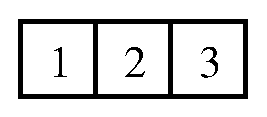
\includegraphics[width=1.5cm,height=1.5cm,keepaspectratio]
 {d3_s.eps}}  
\qquad\qquad
\raisebox{-0.6cm}{
 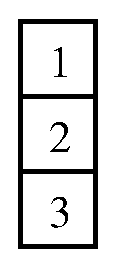
\includegraphics[width=1.5cm,height=1.5cm,keepaspectratio]
 {d3_a.eps}}  
\qquad\qquad
\raisebox{-0.35cm}{
 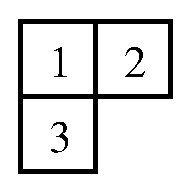
\includegraphics[width=1.0cm,keepaspectratio]
 {d3_t1.eps}} 
\qquad\qquad
\raisebox{-0.35cm}{
 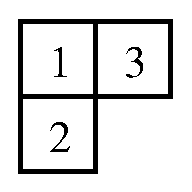
\includegraphics[width=1.0cm,keepaspectratio]
 {d3_t2.eps}}
\end{equation}

	The first diagram corresponds to an absolutely 
	symmetric component of the tensor:
\[
\raisebox{-0.1cm}{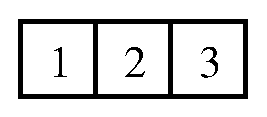
\includegraphics[width=1.5cm,height=1.5cm,keepaspectratio]
 {d3_s.eps}}
	~~\longrightarrow~~
	S^{\mu\nu\rho} ~=~ T^{(\mu\nu\rho)} ~=~
	T^{\mu\nu\rho} ~+~ 	T^{\nu\rho\mu} ~+~	T^{\rho\mu\nu} 
 ~+~	T^{\mu\rho\nu} ~+~ 	T^{\rho\nu\mu} ~+~	T^{\nu\mu\rho}~.
\]
	The second diagram is the absolutely antisymmetric component:
\[
\raisebox{-0.7cm}{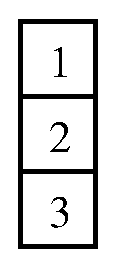
\includegraphics[width=1.5cm,height=1.5cm,keepaspectratio]
 {d3_a.eps}}
	~~\longrightarrow~~
	A^{\mu\nu\rho} ~=~ T^{[\mu\nu\rho]} ~=~
	T^{\mu\nu\rho} ~+~ 	T^{\nu\rho\mu} ~+~	T^{\rho\mu\nu} 
 ~-~	T^{\mu\rho\nu} ~-~ 	T^{\rho\nu\mu} ~-~	T^{\nu\mu\rho}~.
\]
	The two ``corner'' diagrams generate, correspondingly,
\[
\raisebox{-0.4cm}{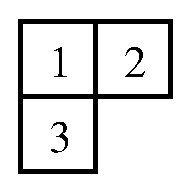
\includegraphics[width=1.0cm,height=1.0cm,keepaspectratio]
 {d3_t1.eps}}
	~~~~\longrightarrow~~~~
	T_1^{\mu\nu\rho} ~=~
	T^{\mu\nu\rho} ~-~ T^{\rho\nu\mu} ~+~ T^{\nu\mu\rho}
	~-~  T^{\rho\mu\nu}~,
\]
	and
\[
\raisebox{-0.4cm}{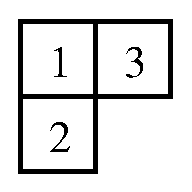
\includegraphics[width=1.0cm,height=1.0cm,keepaspectratio]
 {d3_t2.eps}}
	~~~~\longrightarrow~~~~
	T_2^{\mu\nu\rho} ~=~
	T^{\mu\nu\rho} ~-~ T^{\nu\mu\rho} ~+~ T^{\rho\nu\mu}
	~-~  T^{\nu\rho\mu}~.
\]
	To provide a slightly more complicated example of applying
	the (anti)symmetrization rules we demonstrate
	a diagram corresponding to an irreducible component of a 
	four-tensor:
\[
\raisebox{-0.6cm}{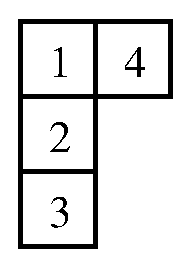
\includegraphics[width=1.5cm,height=1.5cm,keepaspectratio]
 {d4_sample.eps}}
	~~~~\longrightarrow~~~~
	T^{[\mu\nu\rho]\lambda} ~+~ T^{[\lambda\nu\rho]\mu}~.
\]

	All four components of \eqref{rank3_diags} 
	(weighed by appropriate coefficients) sum into
	the original tensor $ T^{\mu\nu\rho} $:
\[
	T^{\mu\nu\rho} ~=~
	\frac{1}{3!}\, \left\lgroup S^{\mu\nu\rho} ~+~
				 A^{\mu\nu\rho} ~+~
				 2 T_1^{\mu\nu\rho} ~+
				 2 T_2^{\mu\nu\rho} \right\rgroup~.
\]
	
	The last step to perform is subtract from each component
	all traces obtained by contraction of any two indices which
	are not antisymmetrized (contraction of antisymmetrized indices is
	trivial).
	The solution can be sought by means of a tensor of a rank
	$ r - 2 $:
\begin{equation}
\label{subtr_traces}
	T_{i\;{\rm (irr)}}^{\mu\nu\rho\lambda...} ~=~
	T_i^{\mu\nu\rho\lambda...}  ~-~  a^{\rho\lambda...}g^{\mu\nu} 
				  ~+~  a^{\rho\mu...}g^{\lambda\nu} ~+~ ...~,
\end{equation}
	where $ T_i^{\mu\nu\rho\lambda...} $ is the $ i $-the component
	obtained from the corresponding Young tableau.
	The traces part in the r.h.s. of \eqref{subtr_traces} should 
	possess the same symmetries as $ T_i^{\mu\nu\rho\lambda...} $
	so as to promote these symmetries to the l.h.s.
	Contracting any two indices in equation \eqref{subtr_traces} and
	requiring the result to vanish one can obtain the explicit expression
	for the trace $ a^{\rho\lambda..} $.


	
\bibliographystyle{apsrev}
\bibliography{class}

	
\end{document}
